% Options for packages loaded elsewhere
\PassOptionsToPackage{unicode}{hyperref}
\PassOptionsToPackage{hyphens}{url}
\PassOptionsToPackage{dvipsnames,svgnames,x11names}{xcolor}
%
\documentclass[
  10pt,
]{scrbook}
\usepackage{amsmath,amssymb}
\usepackage{lmodern}
\usepackage{iftex}
\ifPDFTeX
  \usepackage[T1]{fontenc}
  \usepackage[utf8]{inputenc}
  \usepackage{textcomp} % provide euro and other symbols
\else % if luatex or xetex
  \usepackage{unicode-math}
  \defaultfontfeatures{Scale=MatchLowercase}
  \defaultfontfeatures[\rmfamily]{Ligatures=TeX,Scale=1}
\fi
% Use upquote if available, for straight quotes in verbatim environments
\IfFileExists{upquote.sty}{\usepackage{upquote}}{}
\IfFileExists{microtype.sty}{% use microtype if available
  \usepackage[]{microtype}
  \UseMicrotypeSet[protrusion]{basicmath} % disable protrusion for tt fonts
}{}
\makeatletter
\@ifundefined{KOMAClassName}{% if non-KOMA class
  \IfFileExists{parskip.sty}{%
    \usepackage{parskip}
  }{% else
    \setlength{\parindent}{0pt}
    \setlength{\parskip}{6pt plus 2pt minus 1pt}}
}{% if KOMA class
  \KOMAoptions{parskip=half}}
\makeatother
\usepackage{xcolor}
\IfFileExists{xurl.sty}{\usepackage{xurl}}{} % add URL line breaks if available
\IfFileExists{bookmark.sty}{\usepackage{bookmark}}{\usepackage{hyperref}}
\hypersetup{
  pdftitle={Modeling Mindsets},
  pdfauthor={Christoph Molnar},
  colorlinks=true,
  linkcolor={Maroon},
  filecolor={Maroon},
  citecolor={Blue},
  urlcolor={Blue},
  pdfcreator={LaTeX via pandoc}}
\urlstyle{same} % disable monospaced font for URLs
\usepackage{longtable,booktabs,array}
\usepackage{calc} % for calculating minipage widths
% Correct order of tables after \paragraph or \subparagraph
\usepackage{etoolbox}
\makeatletter
\patchcmd\longtable{\par}{\if@noskipsec\mbox{}\fi\par}{}{}
\makeatother
% Allow footnotes in longtable head/foot
\IfFileExists{footnotehyper.sty}{\usepackage{footnotehyper}}{\usepackage{footnote}}
\makesavenoteenv{longtable}
\usepackage{graphicx}
\makeatletter
\def\maxwidth{\ifdim\Gin@nat@width>\linewidth\linewidth\else\Gin@nat@width\fi}
\def\maxheight{\ifdim\Gin@nat@height>\textheight\textheight\else\Gin@nat@height\fi}
\makeatother
% Scale images if necessary, so that they will not overflow the page
% margins by default, and it is still possible to overwrite the defaults
% using explicit options in \includegraphics[width, height, ...]{}
\setkeys{Gin}{width=\maxwidth,height=\maxheight,keepaspectratio}
% Set default figure placement to htbp
\makeatletter
\def\fps@figure{htbp}
\makeatother
\setlength{\emergencystretch}{3em} % prevent overfull lines
\providecommand{\tightlist}{%
  \setlength{\itemsep}{0pt}\setlength{\parskip}{0pt}}
\setcounter{secnumdepth}{5}
% Geometry
\usepackage[paperwidth=18.9cm, paperheight=24.61cm, inner=30mm, outer=17mm, top=30mm, bottom=24mm]{geometry}


% Decide for a font
%\usepackage{Alegreya}
%\usepackage[scale=.7]{sourcecodepro}


% Make stuff less floaty
\renewcommand{\textfraction}{0.05}
\renewcommand{\topfraction}{0.8}
\renewcommand{\bottomfraction}{0.8}
\renewcommand{\floatpagefraction}{0.75}

% For proofreading: Big margin on the right and 2x linespace
%\linespread{2}
%\geometry{
%  a4paper,
%    total={189mm,246mm},
%  left=20mm,
%  top=20mm,
%  right=70mm,
%  asymmetric
%}

% Header and footer configuration
\usepackage[automark,headsepline]{scrlayer-scrpage}
% Use scrpage2 instead of scrlayer-scrpage if you want to nicer chapter boxes, see main/main.tex. --- WILL NOT WORK WITH TEXLIVE 2019! ----
%\usepackage[automark,headsepline]{scrpage2}
\pagestyle{scrheadings}
\ihead[\headmark]{\headmark}\ohead{\pagemark}
% alternating chapter / section titles at the top of the page
\automark[section]{chapter}
% Make heading of each page italics and small capitals.
\renewcommand*{\headfont}{\itshape\scshape}
% Name of the chapter (\chapapp), number of the chapter (\thechapter) and no period (\autodot)
\renewcommand*{\chaptermarkformat}{\chapapp~\thechapter\autodot\enskip}
% Removes page numbers from bottom
\ofoot{}


% Turns href urls into foodnotes
\let\oldhref\href
\renewcommand{\href}[2]{#2\footnote{\url{#1}}}

% Create index
\usepackage{makeidx}
\makeindex

% Pages for publishing, like empty pages
\frontmatter
\ifLuaTeX
  \usepackage{selnolig}  % disable illegal ligatures
\fi

\title{Modeling Mindsets}
\usepackage{etoolbox}
\makeatletter
\providecommand{\subtitle}[1]{% add subtitle to \maketitle
  \apptocmd{\@title}{\par {\large #1 \par}}{}{}
}
\makeatother
\subtitle{The Many Cultures of Learning From Data}
\author{Christoph Molnar}
\date{2022-04-28}

\begin{document}
\maketitle

%\cleardoublepage\newpage\thispagestyle{empty}\null
%\cleardoublepage\newpage\thispagestyle{empty}\null
%\cleardoublepage\newpage
\thispagestyle{empty}
%\begin{center}
%\includegraphics{images/dedication.pdf}
%\end{center}

%\setlength{\abovedisplayskip}{-5pt}
%\setlength{\abovedisplayshortskip}{-5pt}


% =========================================================================
% Title page with cover
% =========================================================================

\iffalse
\thispagestyle{empty}

\vspace{3cm}
  \begin{center}
    {
	\bfseries \sffamily \Huge Modeling Mindsets for Data Scientists \par
	\bfseries \LARGE The Many Cultures of Learning From Data \par
~\\
	~\\
	\bfseries \small Published by Christoph Molnar, Munich\par
      }
  \end{center}


\newpage
\fi
% =========================================================================
% Page with publishing details
% =========================================================================



\thispagestyle{empty}
\begin{center}
  {
  \bfseries \sffamily \LARGE Modeling Mindsets for Data Scientists \par
  \bfseries \small The Many Cultures of Learning From Data  \par
}

\copyright~2022 \textit{Christoph Molnar}, Germany, Munich\\
\url{christophmolnar.com}

For more information about permission to reproduce selections from this book, write to \url{christoph.molnar.ai@gmail.com}.

	\the\year, Second Edition

% Impression line, indicating number and year of current printing
% International Standard Book Number (ISBN)
% International Standard Serial Number (ISSN), if applicable
\ifxetex
	\textsc{ISBN 9798411463330 (paperback)} 
\fi


\includegraphics{images/by-nc-sa.png}

This book is licensed under the Creative Commons Attribution-NonCommercial-ShareAlike 4.0 International License.
% For translations, indication of original-language title, publisher, and copyright, acknowledgments, permissions, and other credits, including acknowledgment of grants, if applicable and space permitting
  
  Christoph Molnar,
  c/o Mucbook Clubhouse,
  Westendstraße 78,
  80339 München, Germany

\end{center}

% =========================================================================
% Dedication / Empty page before outline
% =========================================================================
\newpage
\thispagestyle{empty}
\mbox{}
\newpage








{
\hypersetup{linkcolor=}
\setcounter{tocdepth}{1}
\tableofcontents
}
\hypertarget{summary}{%
\chapter*{Summary}\label{summary}}


We use data to advance science, make businesses more profitable, automate annoying tasks, and develop smart products.
But there is a middleman between data and its usefulness: the \textbf{model}.
The model that was learned from data represents a simplified aspect of the world; it's the glue that connects data and world.

Statistics versus machine learning, frequentist versus Bayesian inference, causation or association, \ldots{}
There are many mindsets to consider for building models from data.
Each of these modeling mindsets has its own assumptions, strengths, and limitations.

The best modelers, researchers, and data scientists don't stubbornly stick to just one mindset.
The best modelers mix and match the mindsets.

It can take years to truly grasp a new mindset.
Most books and courses jump right into math and methods instead of discussing the fundamental mindset.
But learning a new mindset doesn't have to be this difficult.

The Modeling Mindset book introduces all the cultures of learning models from data.
Each of them enhances your own mind and makes you a better modeler:

\begin{itemize}
\tightlist
\item
  Frequentist inference: learning about nature's ``true'' values.
\item
  Bayesian inference: updating your beliefs about the world.
\item
  Supervised machine learning: predicting new data well.
\item
  Causal inference: taking causality seriously.
\item
  Deep learning: embedding the world into a neural network.
\item
  And many more.
\end{itemize}

Modeling Mindsets opens the door to all these different ways of thinking.
The book is packed with intuitive explanations and striking illustrations.
Quickly get an overview of the strengths and the limitations of each modeling mindset.
Expand your mind when it comes to modeling the world using data.

\hypertarget{what-this-book-is-about}{%
\chapter{What This Book is About}\label{what-this-book-is-about}}

The book is about all the different mindsets that allow you to model the world with data.
Each mindset represents a different perspective on how to see the world through data.
In this book, you will find for each mindset the \textbf{assumptions, central ideas, their relationship to other mindsets, and their strengths and limitations}.
Modeling mindsets is not about history.
Modeling mindsets is a mixture of lightweight methodological introduction and philosophy.
That said, this book is not and \textbf{cannot be a full introduction to each mindset}.
There are entire books about, for example, Bayesian inference, or supervised machine learning.
After reading this book, you will not automatically become a frequentist statistician, or a causal inference expert.
Sorry to disappoint this early in the book.
However, reading Modeling Mindsets can open doors to new ways of thinking about modeling.
But there are other resources to explore what's behind each door -- an online course on machine learning, blog posts about about causal inference, a book about design-based inference, \ldots{}
In each chapter, I refer to \textbf{useful resources to deepen the particular mindset}.

\hypertarget{who-this-book-is-for}{%
\section{Who This Book is For}\label{who-this-book-is-for}}

The book is for data scientists, statisticians, machine learner, quantitative researchers, \ldots{}
In short, for anyone who already has experience with modeling data.
This means you should probably \textbf{know at least one of the mindsets}.
Perhaps, like me, you studied frequentist statistics.
Or you may be a researcher who has learned to use Bayesian inference to analyze your data.
Or maybe you are a self-taught machine learner.

That said, it's crucial that you don't cling to the mindset you already know.
Let go of the rigid assumptions you've learned.
Open your mind to fundamentally new ways of modeling data.

A little math shouldn't scare you either.
But I can promise you that the book is not too heavy on the math side.

\mainmatter

\hypertarget{models}{%
\chapter{Models}\label{models}}

You gaze at the screen.
The screen shows a table with some data.
Based on this data, you are to answer some questions.
These questions could be:

\begin{itemize}
\tightlist
\item
  Which patients might get side effects from a certain drug?
\item
  How do bee hives react to a change in climate?
\item
  Which supermarket products are often out-of-stock?
\end{itemize}

In the data you can see in detail what happened: patients with ID 124 and 22 got acne; 2/3 of bee colonies had trouble during drought in 2018; on that one Tuesday the flour was sold out;
But with data, you can't immediately see general rules and relationships.
Is flour generally in low supply at the beginning of the week?
It would be even better if these rules and relationships applied not only to your specific data sample, but to a more general population of patients/hives/supermarkets.
To move from data to generalizable relationships, we have to simplify the world and make assumptions.
The end result is a model of the world based on data.

A model is a simplified representation of some aspect of the world.
For example, how bee colonies depend on climate.
With a model we can answer questions and make predictions that we couldn't with the raw data.

In this book, we talk about certain types of models:
Models must be computational or mathematical models.
This excludes, for example, physical models, like the tiny houses that architects build.
The second restriction: The models are learned from data.
This excludes ``designed'' models such cellular automata.

There is no philosophical consensus on what makes a model.
For our purpose, let's say that \textbf{a mathematical model consists of three ingredients: variables, relations and parameters}.
A mathematical model contains mathematical structures that represent \emph{variables} and put them in \emph{relation} (Figure \ref{fig:model}). \footnote{Weisberg, Michael. Simulation and similarity: Using models to understand the world. Oxford University Press, 2012.}
The relations are often expressed as parameterized functions of the variables.
The model \textbf{parameters} make the mathematical structure adaptable.
When the model is learned from data, in the learning process the parameters and sometimes relations (functions) are adapted to the data.
If you want to interpret models instead of the world, you have to make assumptions about the relationship between the model and aspects of the world.
But more about this in the chapter \protect\hyperlink{mindsets}{Mindsets}.

\begin{figure}

{\centering 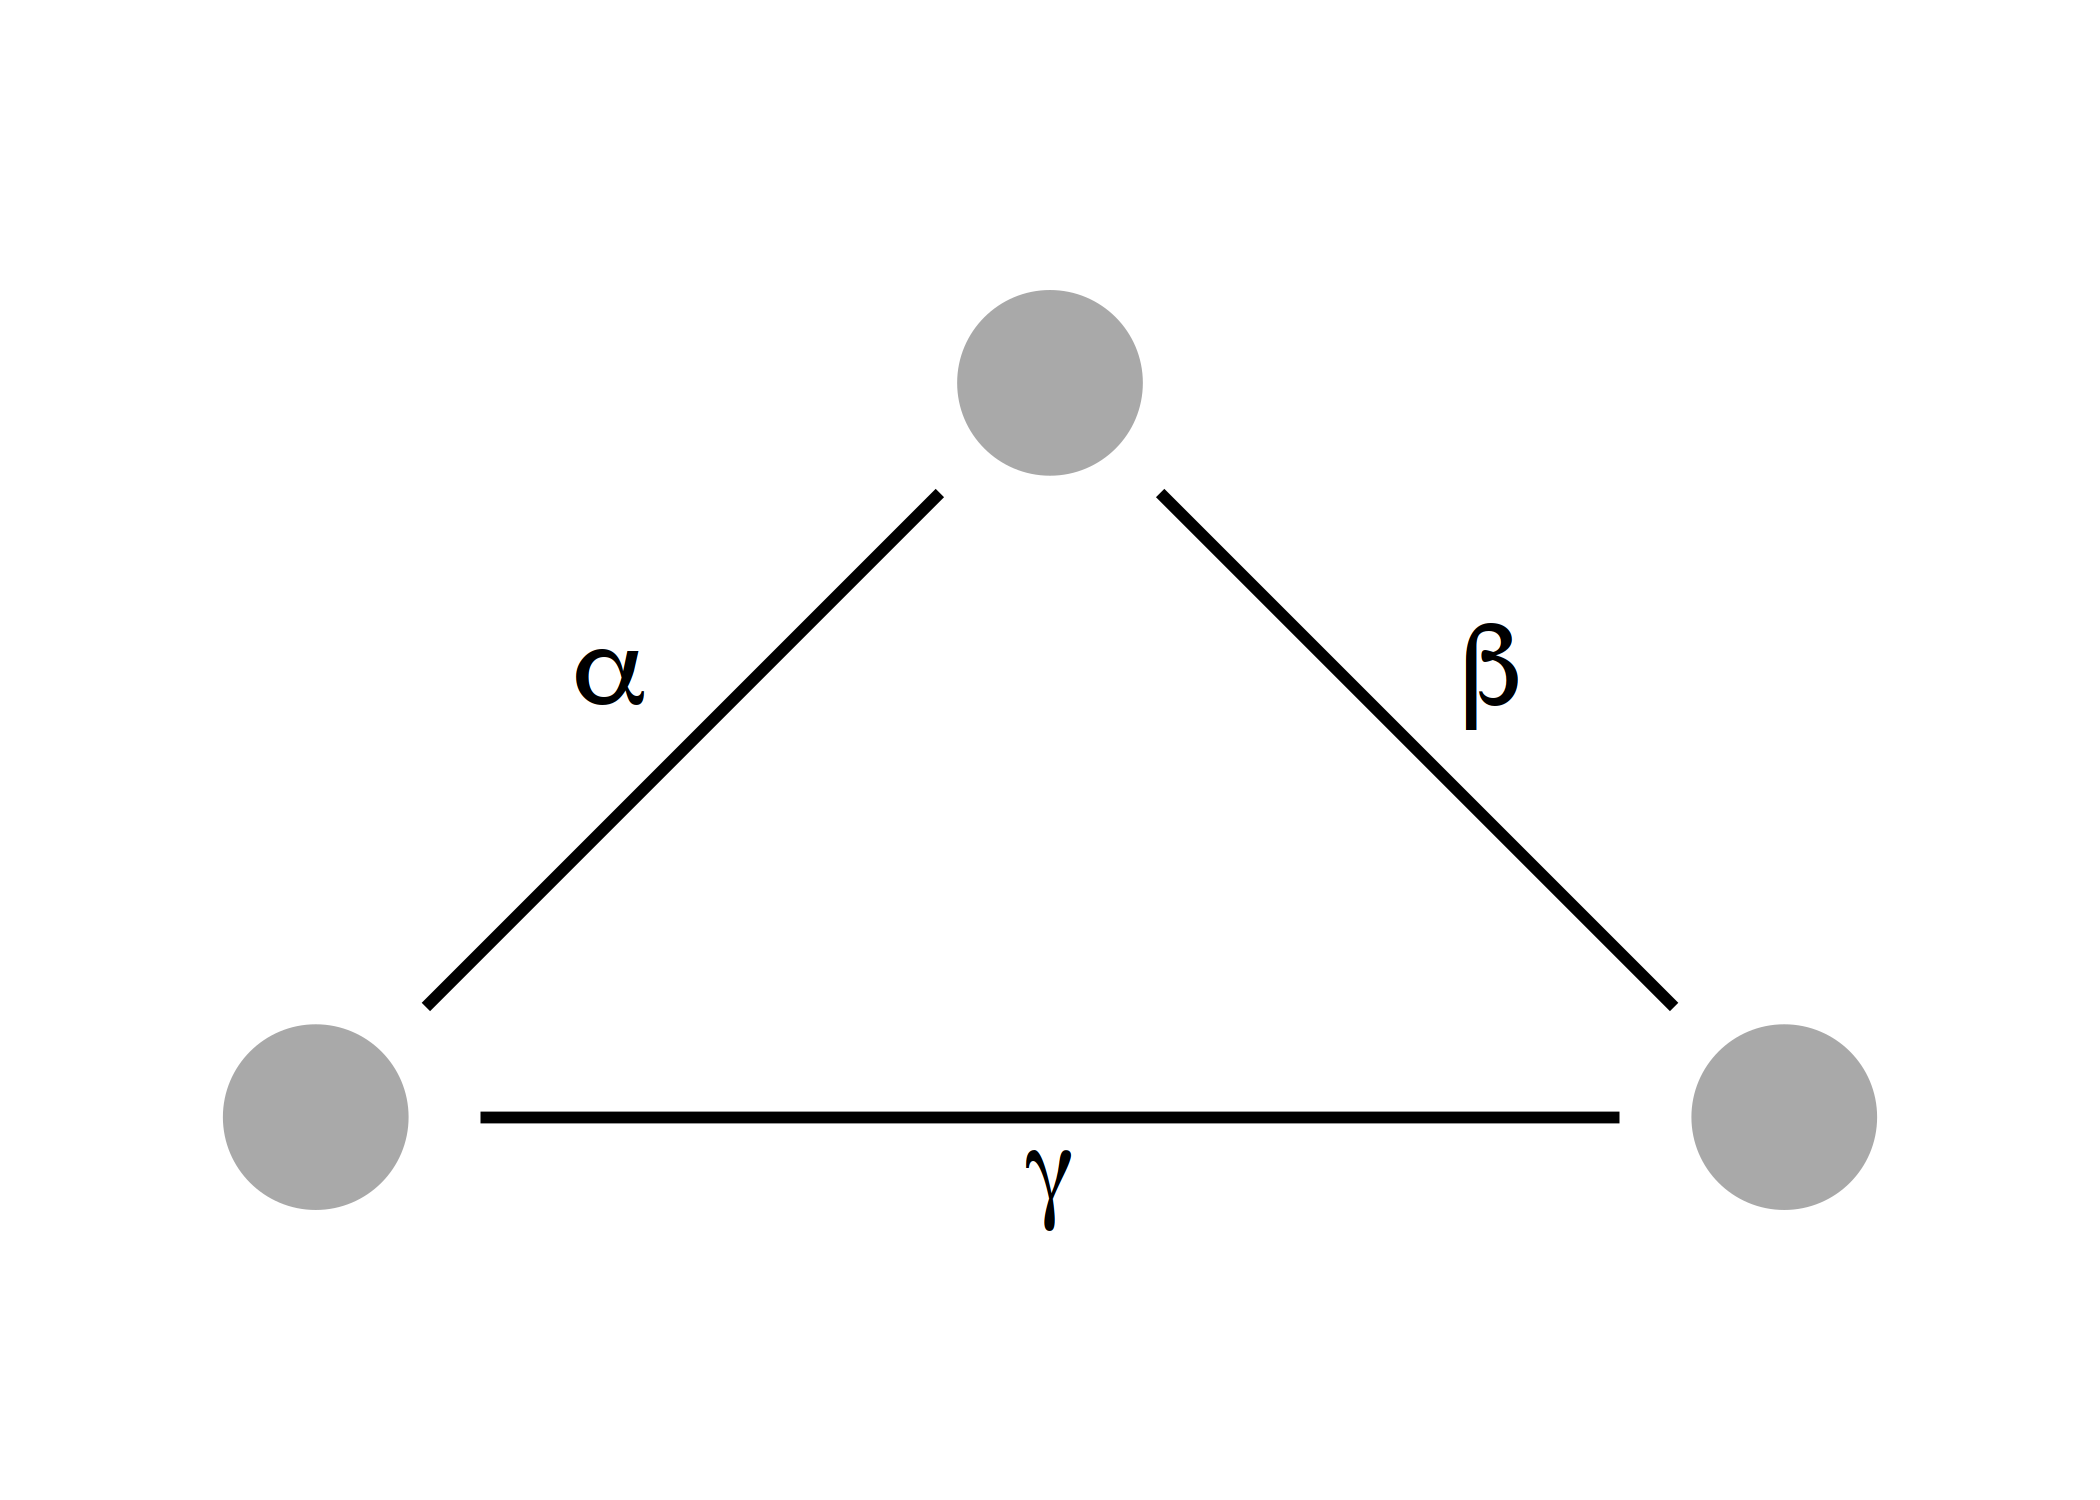
\includegraphics[width=0.8\textwidth]{figures/model-1} 

}

\caption{A mathematical model sets variables (dots) into relation (lines) using parameters.}\label{fig:model}
\end{figure}

The aspects of the world are represented within the model as \emph{variables}.
The blood pressure of a patient is represented with a numerical value.
Images, for example, are represented as tensors of pixels.
Variables can also represent a latent, hidden or abstract aspect.
Like happiness or introversion.
There are different names for variables:
Random variables, covariates, predictors, latent variables, features, target, outcome, \ldots{}
These names sometimes reveal the role of a variable in the model.
For example, the ``target'' is the variable that we want to predict.
In different mindsets, variables have different names and roles:
In machine learning, for example, the terms feature and target are used.
In statistics, people might say dependent and independent variable or covariates and outcome instead.

Within the model, the components are mathematically or computationally set in \emph{relation} to each other.
These relations are usually expressed as parameterized functions.
For example:

\begin{itemize}
\tightlist
\item
  Causal models represent relations between variables in a directed acyclic graph that can be translated into conditional (in-)dependencies.
\item
  The joint distribution of variables describes the occurrence of certain variable values in a probabilist sense.
\item
  A predictive model represents the output variable as a parameterized function of the input variables.
\item
  In the case of a linear regression model, the output variable is a weighted sum of the input variables.
\end{itemize}

The expressive power of such relationships really depends on the class of the model.
A relation can be a simple linear equation like \(Y = 5 \cdot X\) involving two or more variables.
For example we might model the probability of a stroke as a function of blood pressure and age.
A relation can also be a long chain of mathematical operations involving thousands of variables.
Deep neural networks are an example of such a complicated relation.

We don't know the relations between variables in advance, so we use data to learn them.
For some models, learning these relationships is a matter of finding the right \emph{parameters}.
This is true for neural networks and generalized additive models, for example.
For other models, the model structure is ``grown'', as in decision trees or support vector machines.
Growing the structure means not only learning parameters, but also learning the structure of the mathematical function.

You can think of a model as having an uninstantiated state and an instantiated state.
An uninstantiated model is not yet fitted to the data.
Uninstantiated models form families of models.
For example the neural network ResNet architecture, or the family of Poisson regression models.
An instantiated model is trained / learned / fitted using data: It's parameterized and/or the structure has been learned.

I can buy carrots with money.
How many grams of carrots can I get for 1 euro?
Let's call this unknown parameter in our equation \(\beta\):
\(1 \text{ EUR} = \beta \text{ Carrots}\).
I could figure out the \(\beta\) by going to the supermarket and checking the price.
Maybe \(\beta = 500\), so I get half a kilogram of carrots for 1 euro.
But that's only for one supermarket!
Maybe I have to add more variables and relations to the model.
Maybe I need to consider the supermarket chain, special deals, organic / non-organic, \ldots{}
All these choices add variables, relations and parameters to the model.

What we can do with the model depends on the modeling mindset.
In supervised machine learning, we take advantage of the modeled relations to make predictions.
In causal inference, we use our model to estimate causal effects.
In likelihoodism, we can compare the likelihoods between models.

\hypertarget{mindsets}{%
\chapter{Mindsets}\label{mindsets}}

A model is only a bunch of variables, relations, and parameters.
A model alone can't tell us how to interpret the world.
The use and interpretation of the model depends on the mindset from which the model arose.
In order to derive knowledge about the world from the model, we need to make further assumptions.
Consider a linear regression model that predicts regional rice yield as a function of rainfall, temperature, and fertilizer use.
It's a model, not a mindset.
How may we interpret the model?
Can we interpret the effect of fertilizer as causal to rice yield? Or is it just a correlation?
Would we trust the model to make accurate predictions for the future as well?
Can we say anything about the statistical significance of the effect of the fertilizer?
Or have we just updated prior information about the effect of fertilizer with new data?

Welcome to \textbf{Modeling Mindsets}.

A modeling mindset is a specification of how to model the world using data.
Modeling mindsets are like different lenses.
All lenses show us the world, but with a different focus.
Some lenses magnify things that are close, some that are far away.
Some glasses are tinted so you can see in bright environments.
When you look through a lens, you see the world in a certain way.
With different modeling mindsets, you can look at the modeling task, but the model will focus on different things.
Bayesianism, frequentism, supervised machine learning, generative models, \ldots{} these are all different mindsets when it comes to building models from data.
Mindsets differ in how they interpret probabilities -- or whether probabilities are part of the language at all.
While mindsets cover many different modeling tasks, they have some tasks where they really shine.
Each mindset invites you to ask different questions, and so shapes the way you view the world through your model.
In supervised machine learning, for example, everything becomes a prediction or classification problem, while in Bayesian inference, the goal is to update our beliefs about the world using probability theory.

\begin{figure}

{\centering 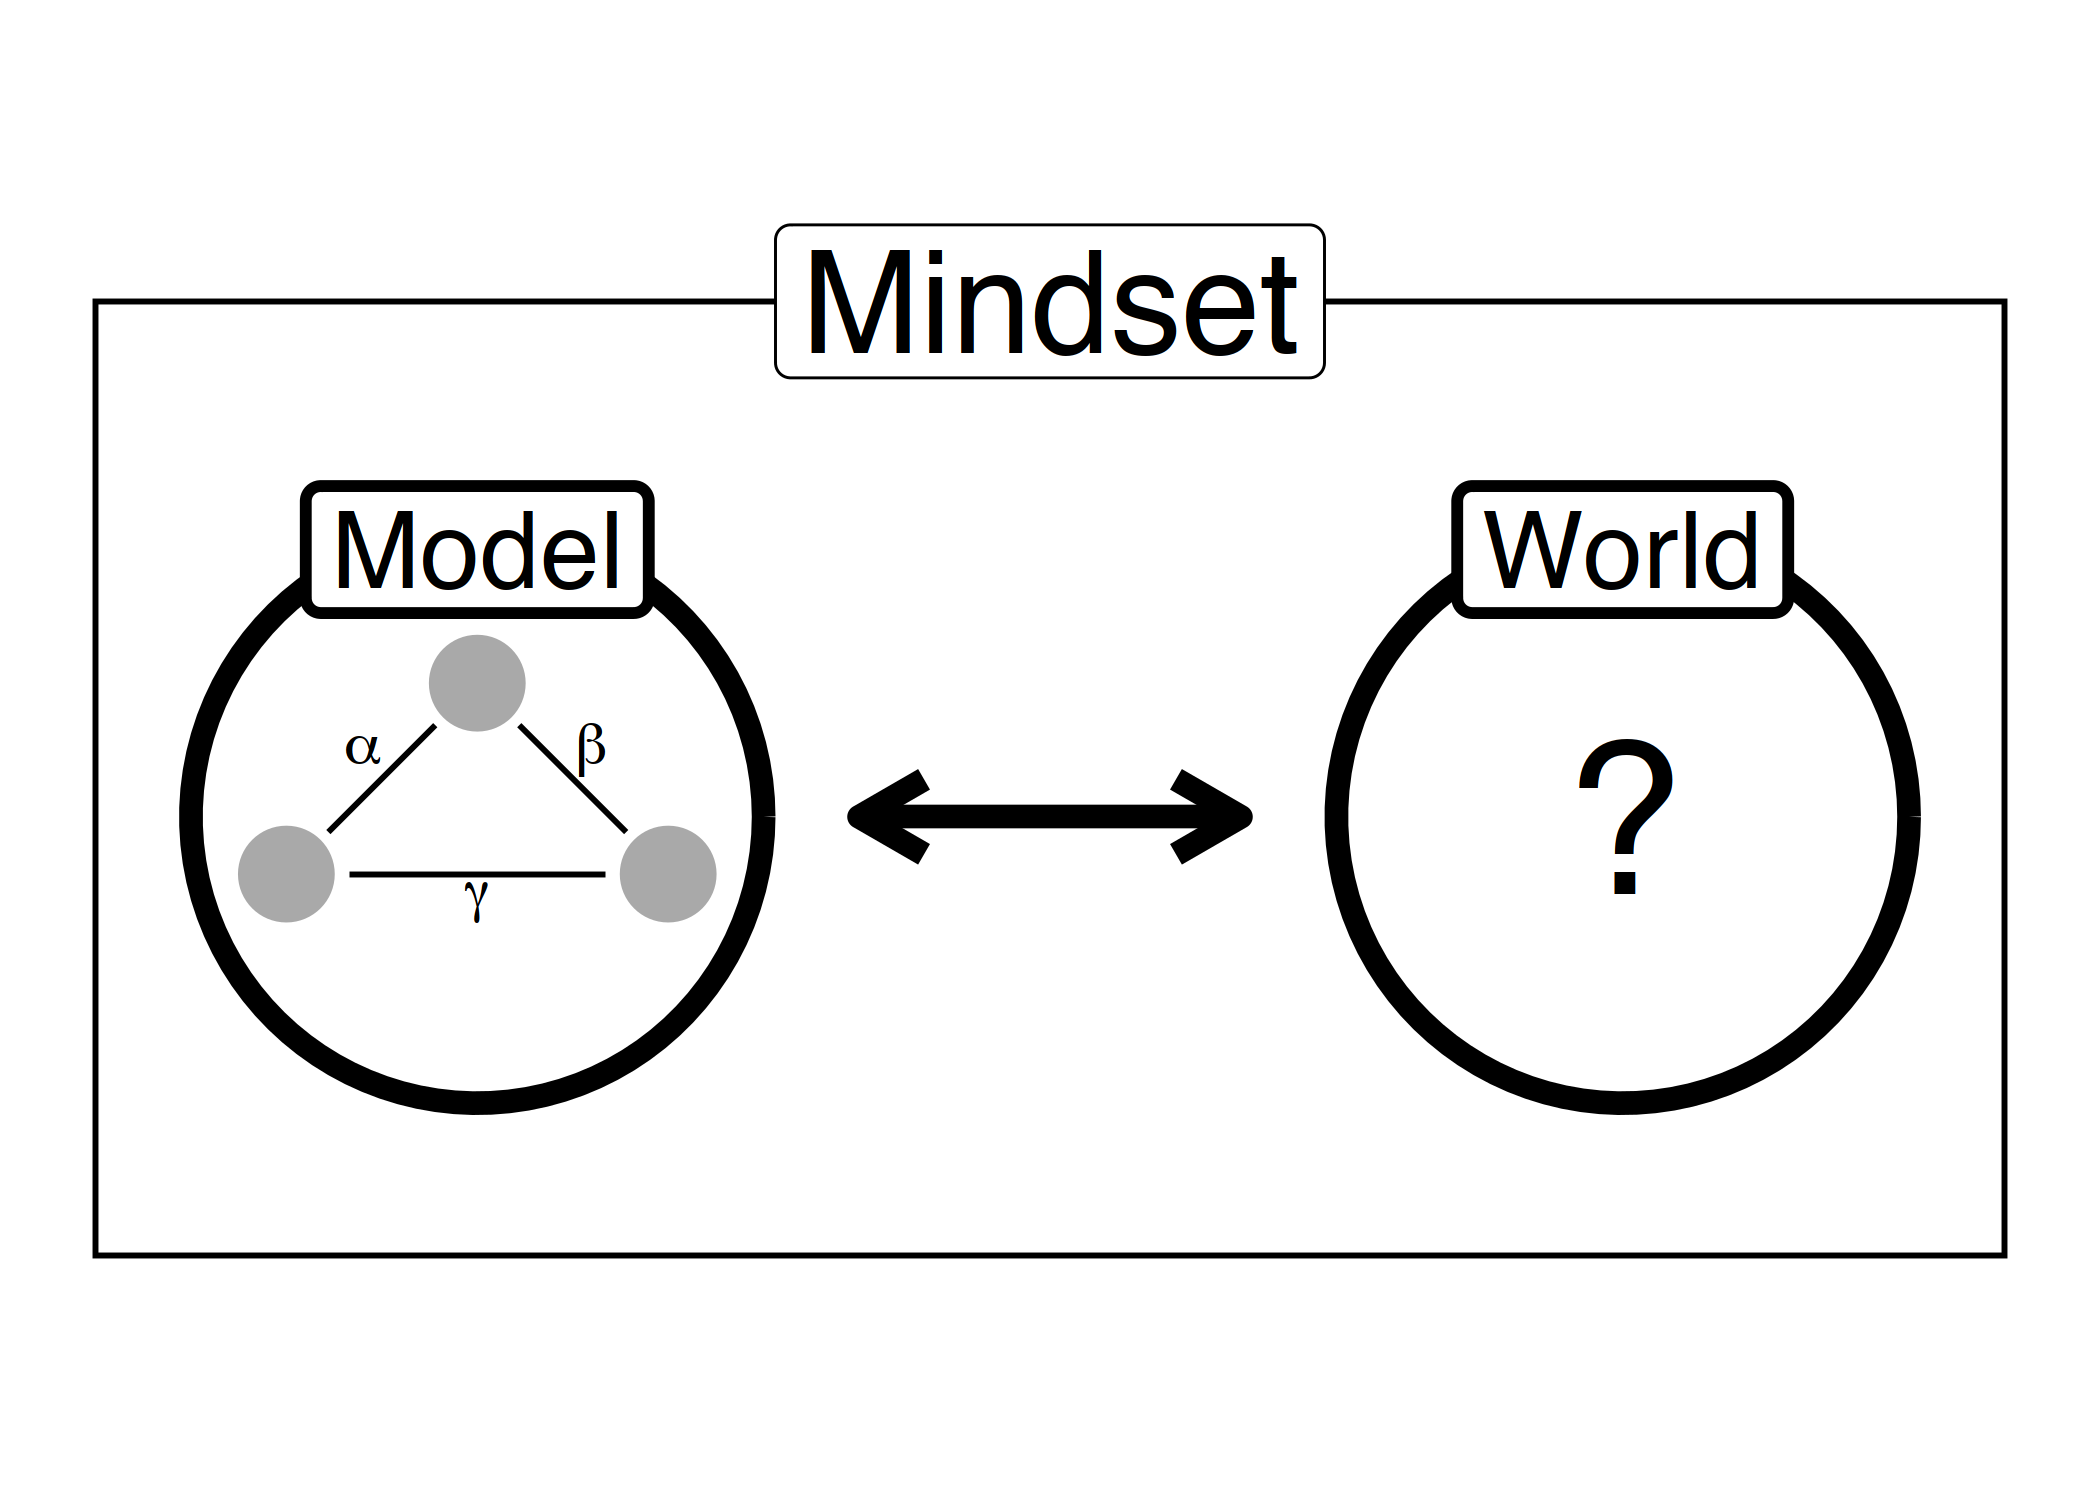
\includegraphics[width=0.8\textwidth]{figures/mindset-1} 

}

\caption{Only when a model is embedded in a mindset can we put it into context with the world.}\label{fig:mindset}
\end{figure}

\textbf{Modeling mindsets} are normative:
A modeling mindset distinguishes between good and bad models.
Even though model evaluations are partly based on objective criteria, the choice of a criterion is subjective.
Each mindset has their own set of accepted models and evaluation procedures.

For a frequentist statistician, a good model of the world is probabilistic and has a high goodness-of-fit to the data.
The residual errors of the model also pass diagnostic checks.
The frequentist rejects the use of prior probabilities as they appear to be subjective.
The frequentist would also not switch to a random forest just because it has a lower mean squared error on test data.
And why would the statistician switch?
From their point of view, the random forest is a poor model of the world.
We learn nothing about the probability distribution of our variables.
We can't do frequentist hypothesis testing of the effects of variables.
The performance of the frequentist's model on unseen test data is not as important to the frequentist.

A modeling mindset limits the questions that can be asked.
Consequently, some questions or tasks are out of scope of the mindset.
Often the questions are out of scope because they just don't make sense in a particular modeling mindset.
Supervised machine learners formulate tasks as prediction or classification problems.
Questions about probability distributions are out of reach since the mindset is: choose the model that has the lowest generalization error given new data.
So the best model could be any function, such as the average prediction of a random forest, a neural network, and a linear regression model.
If the best model can be any function, questions that a statistician would normally ask (hypothesis testing, parameter estimation, \ldots) become irrelevant to the machine learner.
In machine learning, the best models are usually not classical statistical models.
If the machine learner started asking questions a statistician would ask, they would have to choose a suboptimal model, which is a violation of the mindset.

\textbf{Modeling mindsets are cultural}.
Modeling mindsets are not just theories; they shape and are shaped by communities of people who model the world based on the mindset.
In many scientific communities, the frequentist mindset is very common.
I once consulted a medical student for his doctoral thesis.
I helped him visualize some data.
A few days later he came back, ``I need p-values with this visualization.''
His advisor told him that any data visualization needed p-values.
His advisor's advice was a bit extreme, and not advice that a real statistician would have given.
However, it serves as a good example of how a community perpetuates a certain mindset.
Likewise, if you were trying to publish a machine learning model in a journal that publishes mostly Bayesian analysis, I would wish you good luck.
And I'd bet 100 bucks that the paper would be rejected.

The people within a shared mindset also accept the assumptions of that mindset.
And these assumptions are usually not challenged, but mutually agreed upon
At least implicitly.
If you work in a team that has been using Bayesian statistics for some time, you won't be questioning each model anew about whether using priors is good or whether the Bayesian interpretation of probability is legit.
In machine learning competitions, the model with the lowest prediction error on new data wins.
You will have a hard time arguing that your model should have won because it's the only causal model.
If you believe that causality is important, you would simply not participate.
You can only thrive in machine learning competitions if you have accepted the supervised machine learning mindset.

The modeling mindsets as I present them in this book are archetypes: pure forms of these mindsets.
In reality, the boundaries between mindsets are much more fluid.
These archetypes of mindsets intermingle within individuals, communities and approaches:
A data scientist who primarily builds machine learning models might also use some simple regression models with hypothesis tests -- without cross-validating the models' generalization error.
A research community could accept analyses that use both frequentist and Bayesian statistics.
A machine learning competition could include a human jury who would award additional points if the model is interpretable and includes causal reasoning.

Have you ever met anyone who is really into supervised machine learning?
The first question they ask is ``Where is the labeled data?''.
The supervised machine learner turns every problem into a prediction or classification problem.
Or perhaps you've worked with a statistician who always wants to run hypothesis tests and regression models?
Or you had intense discussion about probability with a hardcore Bayesian?
Some people really are walking archetypes. 100\% of one archetype.
But I would say that most people learned one or two mindsets when they start out.
And later they got glimpses of other mindsets here and there.
Most people's mindset is already a mixture of multiple modeling mindsets.
And that's a good thing.
Having an open mind about modeling ultimately makes you a better modeler.

\hypertarget{statistical-modeling}{%
\chapter{Statistical Modeling}\label{statistical-modeling}}

\begin{itemize}
\tightlist
\item
  Goal: Changing your mind under uncertainty.
\item
  Assumes the world is best described by probability distributions.
\item
  Requires additional assumptions for drawing conclusions. See \protect\hyperlink{frequentism}{frequentism}, \protect\hyperlink{bayesian}{Bayesianism} and \protect\hyperlink{likelihoodism}{likelihoodism}.
\end{itemize}

Do you become more productive when you drink a lot of water?
Is there a fixed ``law'', like a mathematical function, that expresses productivity as a function of water intake?
No.
No, because productivity depends on many factors: sleep duration and quality, distractions, noise pollution, \ldots{}
Because of all these factors and other contingencies, we won't get a perfect equation relating water intake to productivity.
Uncertainty remains.
Even the water intake varies from day to day and from person to person.

Statistics is all about changing your mind under uncertainty.
One way to deal with the uncertainty of the world is to abstract aspects of the world as random variables and ascribe a probability distribution to them.
Daily water intake could be a random variable.
For productivity we would need some clever idea on how to best measure this abstract concept.
A not so clever example: Daily time spent in front of the computer.
To further relate these variables to each other, we can make assumptions on how the data were generated and connect the random variables in a statistical model.

Welcome to the \textbf{statistical modeling} mindset.

A statistical model consists of a set of probability distributions that are fitted to data.
A probability distribution describes the frequency with which we expect to see certain values of random variables.
The second ingredient to a statistical model is the data, from which we estimate those probability distributions.
But let's start with the most elementary unit: the random variable.

\hypertarget{random-variables}{%
\section{Random Variables}\label{random-variables}}

A random variable is a mathematical object that carries uncertainty.
Daily water intake can be a random variable.
Data are seen as \textbf{observations} or realizations of random variables.
If someone drank 2.5 liters of water, that is a realization of the random variable ``daily water intake''.

Other random variables:

\begin{itemize}
\tightlist
\item
  Outcome of a dice roll.
\item
  Monthly sales of an ice cream truck.
\item
  Whether or not a customer has canceled their contract last month.
\item
  Daily amount of rain in Europe.
\item
  Pain level of patients arriving at the emergency room.
\end{itemize}

People with a statistical modeling mindset \textbf{think} in random variables.
Any problem related to data is translated into a set of random variables and solved based on that representation.
A random variable is a construct that we can't observe directly.
But we can observe the realizations of a random variable, as shown in Figure \ref{fig:variable}.
But the raw data are not that useful to humans.
Because humans aren't databases, we need a model that simplifies the noisy data for us.
Statisticians came up with probability distributions: a mathematical construct that describes potential outcomes of the random variable.

\begin{figure}

{\centering 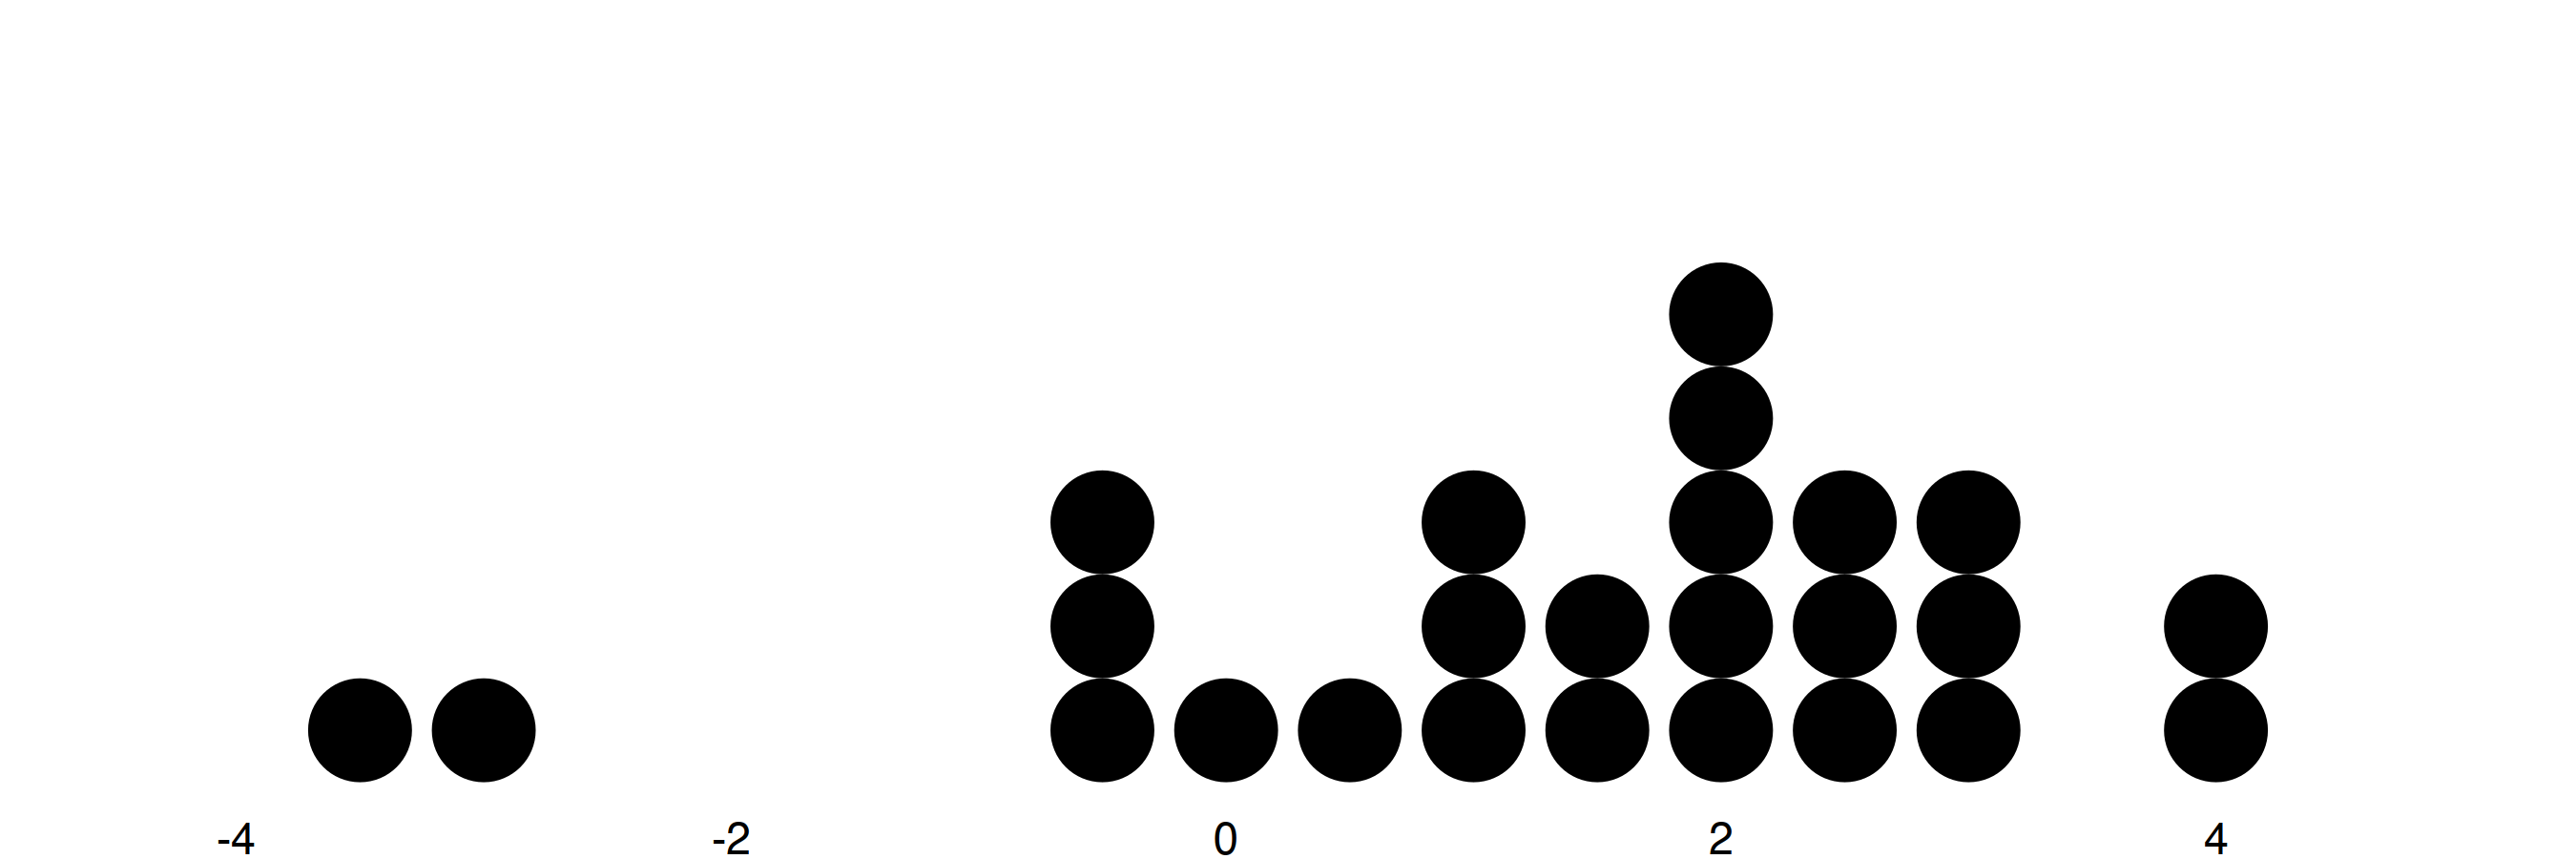
\includegraphics[width=0.8\textwidth]{figures/variable-1} 

}

\caption{Each dot represents a data point, a realizations of a random variable. The x-axis shows the value of the variable. Dots are stacked up for frequently occurring values. }\label{fig:variable}
\end{figure}

\hypertarget{probability-distributions}{%
\section{Probability Distributions}\label{probability-distributions}}

A probability distribution is a function which gives each possible outcome of a random variable a probability.
Value in, probability out.
Not all functions can be used as probability functions.
A probability function must be larger or equal to zero for the entire range of the random variable.
For discrete variables such as the number of fish caught, the probability distribution must sum up to 1 over all possible outcomes.
And for continuous outcomes such as water intake, the probability distribution, also called density function, must integrate to 1 over the possible range of values.

For the outcome \(x\) of a fair dice, we can write the following probability function:

\[
P(x) = 
\begin{cases}
 1/6 & x \in \{1, \ldots, 6\} \\
 0 & x \notin \{1, \ldots, 6\} \\
\end{cases}
\]

The Normal distribution is for continuous variables and defined from minus to plus infinity:

\[f(x) = \frac{1}{\sigma \sqrt{2\pi}} e^{-\frac{1}{2}\left(\frac{x-\mu}{\sigma}\right)^2}\]

In this equation, \(\pi\) and \(e\) are the famous constants \(pi \approx 3.14\) and \(e \approx 2.7\).
The distribution has two parameters: mean \(\mu\) and standard deviation \(\sigma\).
These parameters are sometimes called location (\(\mu\)) and scale (\(\sigma\)) parameters, since they determine where on the x-axis the center of the Normal distribution is and how flat or sharp the distribution is.
The larger the standard deviation \(\sigma\), the flatter the distribution.

Let's try it out and set \(\mu = 0\) and \(\sigma = 1\), as visualized in Figure \ref{fig:distributions}, leftmost curve.
Now we can use this probability distribution function for telling us how probable certain values of our random variable are.
We get \(f(1) \approx 0.24\) and for \(f(2) \approx 0.05\), making \(x=1\) much more likely then \(x=2\).
We may not interpret \(f(x)\) as probability directly.
But we can integrate \(f\) over a region of the random variable to get a probability.
The probability for \(x \in [0.9, 1.1]\) is 4.8\%.

There is huge arsenal of probability distributions: The Normal distribution, the Binomial distribution, the Poisson distribution, \ldots{}
And there is an infinite number of probability distributions that you could invent yourself.

\begin{figure}

{\centering 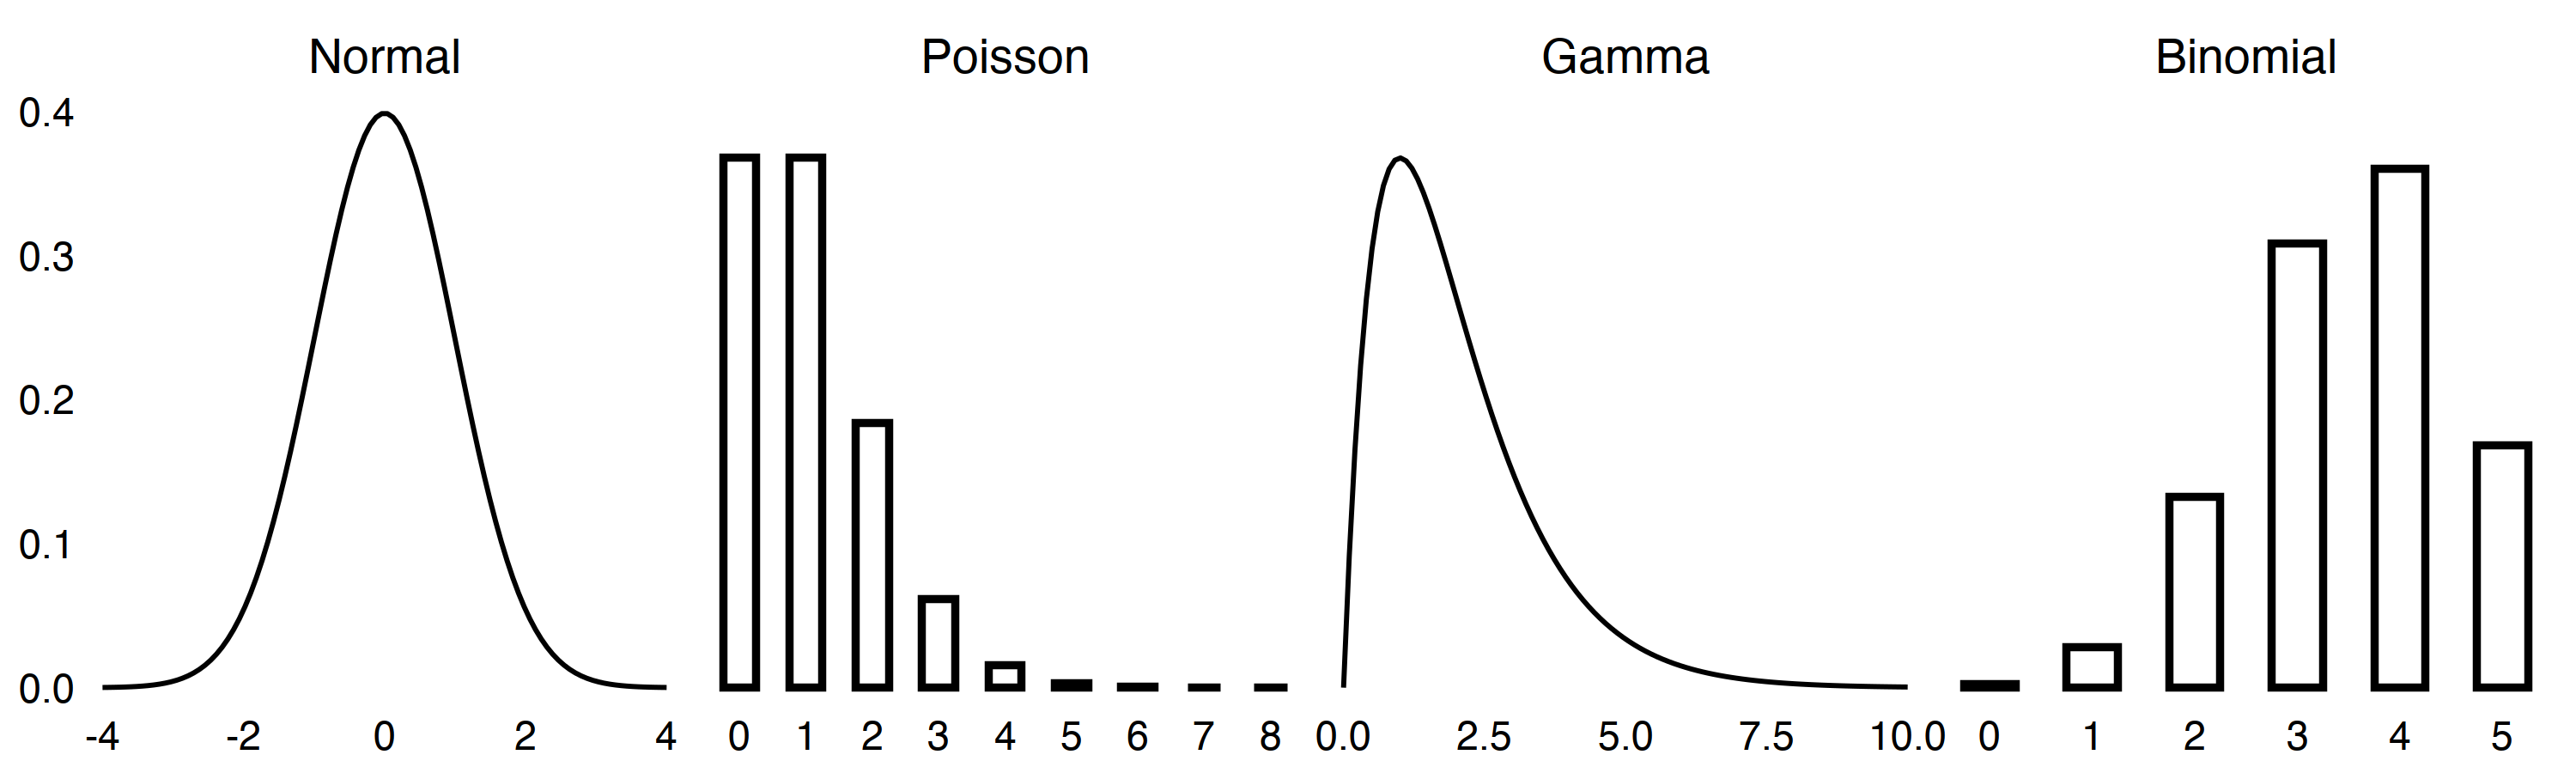
\includegraphics[width=0.8\textwidth]{figures/distributions-1} 

}

\caption{Distributions}\label{fig:distributions}
\end{figure}

\hypertarget{assuming-a-distribution}{%
\section{Assuming a Distribution}\label{assuming-a-distribution}}

An important step in the statistical modeling mindset is to connect the random variables that we are interested in to distributions.
A common approach is to choose a distribution that matches the ``nature'' of your data:

\begin{itemize}
\tightlist
\item
  A numerical outcome such as IQ? That's Normal distribution.
\item
  A count outcome such as number of fish caught in an hour? The Poisson distribution is a solid choice.
\item
  A binary repeated outcome, like the number of successful free throws in basketball? It follows a Binomial distribution.
\end{itemize}

These were examples 1-dimensional distributions that only consider a single variable.
The world is more complex than that:
Random variables can be correlated.
The distribution of one variable can depend on the value that another random variable takes.
Fortunately, it's possible to define so-called multivariate distributions.
A multivariate distribution is a function that takes as input two ore more values and returns a density (still a single number).
We might assume that the joint distribution of water intake and productivity (measured in minutes) follows a 2-dimensional Normal distribution.

Another option is conditional distributions.
For example, we could assume that productivity, conditional on water intake, follows a Normal distribution.

With all these probability distributions, we are still in the realm of abstraction and assumptions.
On one side we have the data: messy and untamed.
On the other side, we have the probability distributions: clean and idealized.
Via random variables we have at least a theory how the two are connected:
The data are the realizations of variables, and distributions summarize the stochastic behaviour of variables.
But we still need to mathematically connect observed data and theoretical distributions.
How can we connect them?

The answer is \textbf{statistical models}.

\hypertarget{statistical-model}{%
\section{Statistical Model}\label{statistical-model}}

A statistical model connects theoretical distributions with observed data.
Statistical models are mathematical models that make assumptions about how the data are generated.
With these assumptions in the background, statistical models are then estimated using data.
More formally, a statistical model is the combination of the sample space from which the data comes from, and a set of probability distributions on this sample space.

The distributions are ``fitted'' to the data by changing the parameters.
Imagine the distribution as a cat.
And your data is a box.
Your cat fits it's shape and position to match the box.

How does the cat know which form to take on?
Ah pardon, our question now is:
How do we find parameter values so that the distribution fits the data well?
The density function of the Normal distribution, for example, has mean and variance as parameters.
Given the parameters, the density or probability function can tell us how likely certain values of our random variables are.

We can also use the probability or density function to find our parameters -- by reversing the point of view and calling it the likelihood function.
The value of the random variable is the input of the probability function, and the parameters are seen as given.
The likelihood function \(L(\theta, X)\) is equal to the probability function.
Except that the parameters are now the input, and the values of the random variable are seen as given.
They are given, in the sense that we have data that are realizations of the random variable.

We can take an observed value for \(X\) from our data and plug it into the likelihood function.
Now we have a likelihood function that can tell us, for this one data point, which parameters would give the highest probability for observed this particular value.
But our data consist of multiple realizations of random variables.
To get the likelihood for the entire dataset, we multiply the likelihoods of the individual data points.
This data likelihood can tell us, for a given parameter value, how likely our data is.
For example we could try \(\mu = 1\) and \(\sigma = 2\) and the likelihood function returns a value.
The larger the value, the better the distribution (with these parameters) fits the data.
That's very useful, because it helps us in finding the best parameters.

Finding the best parameters is a classical optimization problem:
Maximize the data likelihood \(L\) with respect to the parameters.
We want to maximize the likelihood for all of our data: \(L(\theta, \mathbf{x}_1, \ldots, \mathbf{x}_n) = \prod_{i=1}^n L_i(\theta, \mathbf{x}_i)\).
Note that \(\mathbf{x}_i\) can be a vector with values for multiple variables.
And we maximize the data likelihood:

\[\arg \max_{\theta} L(\theta | \mathbf{x}_1, \ldots, \mathbf{x}_n)\]

\hypertarget{maximum-likelihood-estimation}{%
\subsection*{Maximum Likelihood Estimation}\label{maximum-likelihood-estimation}}


Maximum likelihood estimation is a classic optimization problem.
For simpler cases this can even be solved analytically.
For the Normal distribution, we know that the optimal \(mu\) is the mean of the data: \(\frac{1}{n} \sum_{i=1}^n x_i\).
When an analytical solution is not possible, other optimization methods like gradient descent, the Newton-Raphson method and Fisher's scoring can be used.

Maximum likelihood estimation is a key element to understanding the statistical modeling mindset.
Maximizing the likelihood means bringing together the theoretical probability distributions and the observed data.

\begin{figure}

{\centering 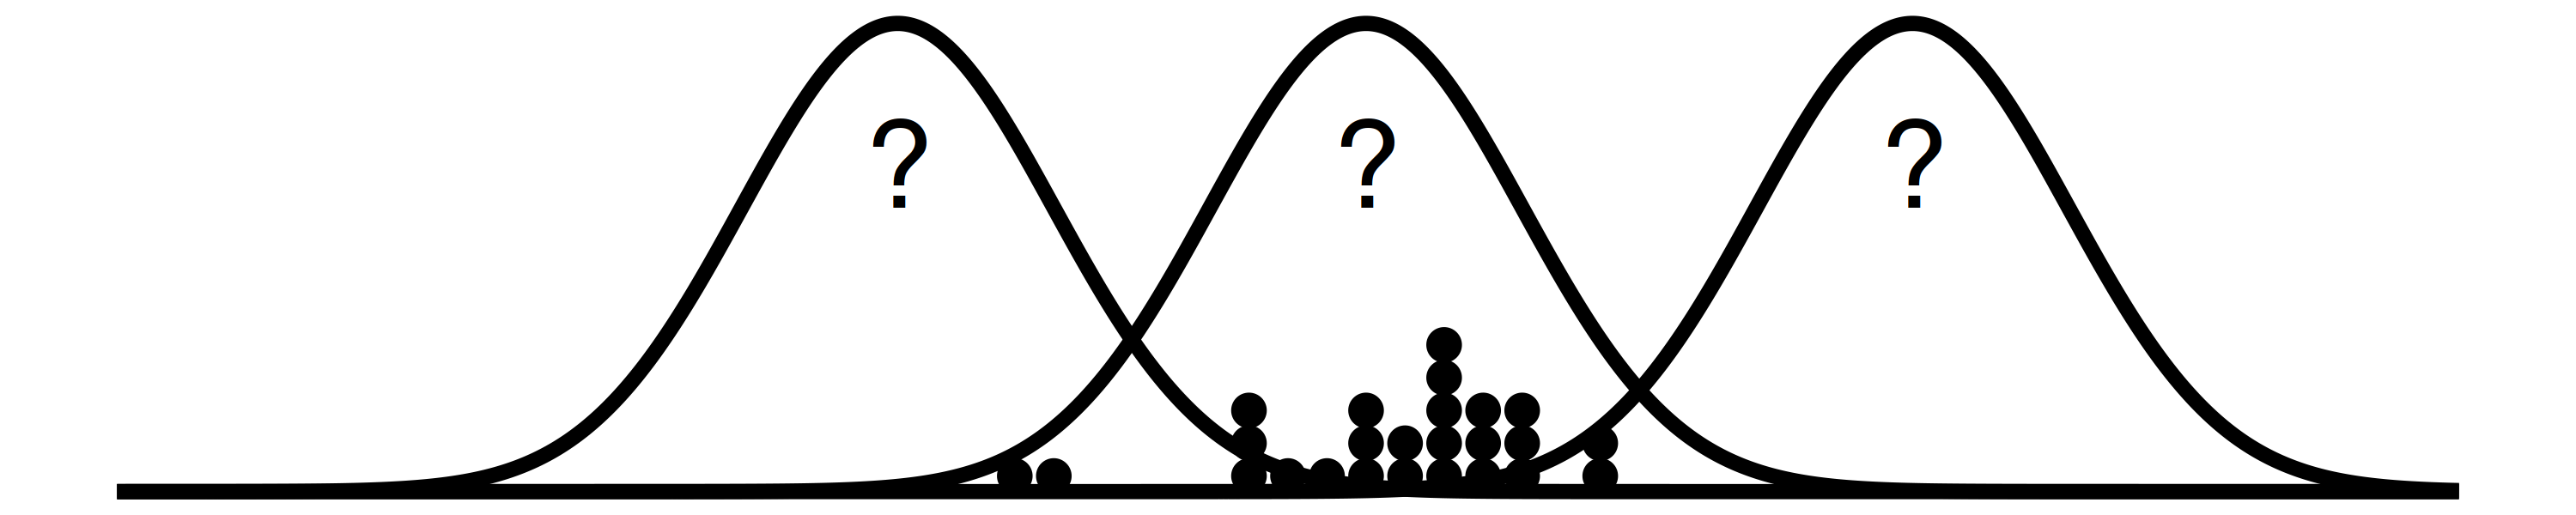
\includegraphics[width=0.8\textwidth]{figures/fit-1} 

}

\caption{Fitting distributions to data}\label{fig:fit}
\end{figure}

\hypertarget{interpreting-parameters}{%
\subsection*{Interpreting Parameters}\label{interpreting-parameters}}


The parameters are not only things to be optimized.
Their role goes beyond that of a mere technical controller.
The parameters are central to the statistical modeling mindset.

\textbf{Statisticians interpret the parameters as summary of the data.}

Statistical modeling is about understanding our data better.
The nice consequence of modeling the data with probability distributions is that we summarize our data with just a few numbers, the parameters.
In the case of the Normal distribution, we can describe the distribution of a single variable with only two numbers, the mean and the standard deviation.
Also for other types of statistical models, parameters are central to interpretation.

\hypertarget{joint-or-conditional-distribution}{%
\section{Joint or Conditional Distribution}\label{joint-or-conditional-distribution}}

All statistical models target an aspect of a probability distribution.
For most of the chapter, we talked about simpler cases, like the distribution of a single variable: \(P(X)\).
But we could have the case of multiple random variables \(X_1, \ldots, X_p\).
To describe the full distribution of more than one variable, we have to work with the joint distribution.

A Gaussian mixture model, for example, requires learning the entire distribution of multiple variables.
Gaussian mixture models can be used for identifying clusters in the data, which are assumed to stem from a mixture of Normal distributions.
Gaussian mixture models are also an example of using a different optimization algorithm than the maximum likelihood algorithm: the expectation-maximization algorithm, which iteratively jumps between optimizing the model parameters and predicting the ``mixture'' of cluster centers for each data point.

The joint distribution is not always of interest and can be difficult to estimate.
It's often much simpler to work with \emph{conditional distributions}.
The conditional distribution tells us how likely the outcome of one or more random variables is given that we already know the values of some other random variables.
For example:

\begin{itemize}
\tightlist
\item
  Which risk factors influence the probability of getting lung cancer?
\item
  How do climatic conditions like temperature and humidity affect the occurrence of bonobos?
\item
  On what days is a hospital likely to be understaffed?
\end{itemize}

The conditional distribution is the natural form for prediction tasks.
And it's usually simpler to estimate than the joint distribution.
Models of the conditional distribution are central to statistical modeling.
They are also known as regression models.

\hypertarget{regression-models}{%
\section{Regression Models}\label{regression-models}}

Regression models are statistical models of the conditional and not the joint distribution.
Let's say we have two variables: \(Y\) and \(X\).
With the joint distribution \(P(Y,X)\) we could answer ``How likely is it that \(X=x\) and \(Y=y\) occur together?
But with the conditional distribution we can ask:''Given \(X=x\), how likely are certain values for \(Y\)``?

For example, we want to know not only how often a disease is successfully treated.
We might want to know if a certain drug played a part in the disease outcome.
Other factors such as the patient's age, disease progression, etc. may play a role.

Our target is the distribution of outcome variable \(Y\) conditional on variables \(X_1, \ldots, X_p\).
Within the regression model, the distribution of \(Y\) is linked to the variables \(X_1, \ldots, X_p\).
Often this means that we express the parameters \(\theta\) of \(Y\)'s distribution (such as the mean \(\mu\) in a Normal distribution) as a function of the other variables.
How exactly this link looks like depends on the distribution that the modeler assumed for \(Y\) and the link they chose to connect \(\theta\) and \(X\).
The simplest case is a linear regression model.
We assume that \(Y\) follows a Normal distribution and link the mean of \(Y\)'s distribution to a weighted sum of the other variables:

\[Y \sim N(\mu, \sigma)\]

\[\mu = \beta_0 + \beta_1 X_1 + \ldots + \beta_p X_p\]

The linear regression model expresses the mean of the target \(Y\) as the weighted sum of the other variables.
\(Y\) given \(\mathbf{X}\) follows a Normal distribution.
We only link the mean \(\mu\) to the variables.
A typical assumption is that the standard deviation \(\sigma\) is independent of the value of the other variables.

What can we do now with a regression model?
We can make predictions.
We just have to fill in values for \(X\) and get the expected value of the probability distribution of \(Y\).
While the conditional mean of \(Y\) is often the goal of the regression model, the statistician can also target other parts of the conditional distribution.
For example the median or other quantiles.
These types of regression models are quantile regression models.
For survival models the target is often the hazard rate, which is a function of the probability of an event happening in a time interval.
See for example the Cox proportional odds model.

\textbf{Interpretation of parameters} is usually even more important than prediction.
The parameters contain information about the relationship between the target and the other variables.
For regression models, we usually speak of the coefficients.
In the linear regression model, a positive coefficient \(\beta_j\) means that increasing the value of variable \(X_j\) increases the expected value of \(Y\).

A large part of statistical modeling consists of regression models in different flavors.

\begin{itemize}
\tightlist
\item
  Generalized linear models (GLMs)
\item
  Generalized additive models (GAMs)
\item
  Quantile regression
\item
  Mixed effect models
\item
  \ldots{}
\end{itemize}

Most of these models were ``invented'' to address a shortcoming of another regression model.
GLMs can model targets that don't follow a Normal distribution but some other distribution.
GAMs can model non-linear relationships.

Regression models also have a place in \protect\hyperlink{mindset}{supervised machine learning}.
But in supervised machine learning, the goal is to achieve good predictive performance on unseen data.
And if a random forest performs better than a GAM, then the GAM gets thrown out, even if it has nicer statistical properties.

\hypertarget{model-evaluation}{%
\section{Model Evaluation}\label{model-evaluation}}

Good statisticians evaluate their models.
Understanding how this evaluation works will help you better understand the statistical modeling mindset.
It's particularly interesting to see how much the evaluation in the statistical modeling mindset differs from that of \protect\hyperlink{supervised-ml}{supervised machine learning}.
The evaluation of statistical models consists of two parts: \textbf{model diagnostics and goodness-of-fit}.

The role of model diagnostics is to check whether the modeling assumptions were reasonable.
If we have assumed that a random variable follows a Normal distribution, we can check this assumption visually.
For example, with a Q-Q plot.
Another typical assumption is homoscedasticity: The variance of the target is independent of other variables.
Homoscedasticity can be checked visually by plotting the residuals (\(y_i\) minus its predicted value) against each of the other variables.

A model that passes these diagnostics is not automatically a good model.
Statisticians use goodness-of-fit measures to compare models and evaluate modeling choices, such as which variables to have in the model.\\
Typical goodness-of-fit measures are the (adjusted) R-squared, Akaikes Information Criterion (AIC), the Bayes factor, and likelihood ratios.
Goodness-of-fit is literally a measure of how well the model fits the data.
The goodness-of-fit can guide the model building process and decide which model is chosen in the end.

Goodness-of-fit is typically computed with the same data that were used for fitting the statistical models.
This choice may look like a minor detail, but it says a lot about the statistical modeling mindset.
The critical factor here is overfitting: The more flexible a model is, the better it adapts to ALL the randomness in the data instead of learning patterns that generalize.
Many goodness-of-fit metrics therefore account for model complexity, like the AIC or adjusted R-squared.
Compare this to \protect\hyperlink{supervised-ml}{supervised machine learning}: in this mindset, there is a strict requirement to always use ``fresh'' data for evaluation.

\hypertarget{data-generating-process-dgp}{%
\section{Data-Generating Process (DGP)}\label{data-generating-process-dgp}}

A quite central, but fuzzy also topic of the statistical modeling mindset is the data-generating process.
The statistical modeler thinks about the data-generating process all the time.
The data-generating process is a construct, an unknowable ideal of how the data were generated.
The data-generating process produces the unknown distributions that then produce the data.
We observe the data-generating process indirectly through the data.
With data and reflections on the DGP, sometimes together with experts, the statistician tries to decipher the DGP.
Statisticians talk about the DGP all the time, but it remains more of a mental model than a clearly defined concept.
When I was studying statistics, the DGP was mentioned in most lectures.
But I never had a formal lecture on what the DGP is.
It's also difficult to find textbooks, lectures, or blog posts that define what the DGP really is.
It seems to me that the mental model of a DGP is a natural consequence of viewing the world in terms of probability distributions.

The DGP is a powerful idea, even if it's not well defined.
Assuming a DGP encourages you to intellectually dive deep into your data.
Having this image of a DGP in your mind let's you take on the mindset of a detective:
Statisticians are like detectives reconstructing a crime.
You can't observe the crime directly.
But the crime has generated a lot of ``data'' at the scene.
The stats detective then tries to uncover the data-generating process by making assumptions and learning from the observed data.

There is no definition of the data-generating process, so I'll give you a some examples:

\begin{itemize}
\tightlist
\item
  Rolling dice is a data-generating process. A die is symmetric, making each side equally likely. We could factor in the angle of the throw, surface roughness and so on. But the chaotic behaviour of the dice bouncing and spinning across the table makes us disregard all these factors.
\item
  We study the income of computer scientists via a survey. Instead of mindlessly reporting the income distribution, we think about the entire data-generating process: For example, some income values are missing. Are they missing at random? Are higher-income individuals more likely to leave the income answer empty? Are some businesses overrepresented in the survey? Is the sample truly random?
\item
  A research team has collected chest x-ray images of patients with and without COVID-19 for building a COVID-19 prediction model. A closer look at the data-generating process shows: the images not only differ in COVID-19 status, but they come from different data-generating processes. COVID-19 images are often taken with patients lying down because of exhaustion. One of the non-COVID-19 datasets are even children x-ray images.\footnote{Wynants, Laure, Ben Van Calster, Gary S. Collins, Richard D. Riley, Georg Heinze, Ewoud Schuit, Marc MJ Bonten et al.~``Prediction models for diagnosis and prognosis of covid-19: systematic review and critical appraisal.'' bmj 369 (2020).} Considering the DGP casts doubt on whether such data can be used to build a COVID-19 classifier or whether, in reality, it classifies data into child/adult, standing/lying down, \ldots{} I chose this example because it's a paper from the \protect\hyperlink{supervised-ml}{supervised machine learning mindset}. A good statisticians would check the DGP much more carefully, making it more likely to detect such problems.
\end{itemize}

If these examples of data-generating processes sound like common sense to you, it's because they are.
But it's surprisingly uncommon among non-statistician mindsets.
For example, for \protect\hyperlink{supervised-ml}{supervised machine learning}, considerations of the data-generating process play a subordinate .
For most machine learning competitions the winner is determined solely by the lowest prediction error on new data.
It doesn't matter whether the model meaningfully reflects the data-generating process.

\hypertarget{drawing-conclusions-about-the-world}{%
\section{Drawing Conclusions About the World}\label{drawing-conclusions-about-the-world}}

In most cases, statistical models are built for practical reasons:
To make a decision, to better understand some property of the world, or to make a prediction.
These goals require the interpretation of the model instead of the world.
But using the model as a representation of the world isn't for free.
The statistician must consider the representativeness of the data and choose a mindset that allows the findings of the model to be applied to the world.

Considering the data-generating process also means thinking about the representativeness of the data, and thus the model.
Are the data a good sample and representative of the quantity of the world the statistician is interested in?
Let's say a statistical modeler analyzes data on whether a sepsis screening tool successfully reduced the incidence of sepsis in a hospital.
They conclude that the sepsis screening tool has helped reduce sepsis-related deaths at that hospital.
Are the data representative of all hospitals in the region, the country, or even the world?
Are the data even representative of all patients at the hospital, or are data only available from patients in intensive care unit?
A good statistical modeler define and discuss the ``population'' from which the data are a sample of.
\protect\hyperlink{design-based}{Design-based inference} fully embraces this mindset that the data are sampled from a larger population.

More philosophical is the modeler's attitude toward causality, the nature of probability, and the likelihood principle.

\begin{quote}
``It is unanimously agreed that statistics depends somehow on probability. But, as to what probability is and how it is connected with statistics, there has seldom been such complete disagreement and breakdown of communication since the Tower of Babel.''
\end{quote}

-- Leonard Savage, 1972\footnote{Savage, Leonard J. The foundations of statistics. Courier Corporation, 1972.}

Statistical modeling is the foundation for learning from data.
But we need another mindset on top of that to make the models useful.

\protect\hyperlink{frequentism}{Frequentist inference} is the most prominent mindset for inferring properties about the world from statistical models.
Frequentist statistics sees probability as relative frequencies of events in long-run experiments.

\protect\hyperlink{bayesian}{Bayesian inference} is based on an interpretation of probability as a degree belief about the world.
Bayesianism states that the model parameters also have a (prior) distribution.
And the goal of the statistician is to update the prior distribution by learning from data.
The resulting posteriori distributions of the parameters express our belief about the world.

\protect\hyperlink{likelihoodism}{Likelihoodism} is a lesser known modeling mindset. Like Bayesianism, it adheres to the likelihood principle, which states that the likelihood function captures all evidence from the data (which frequentist inference violates).
However, it does not require prior probabilities.

\protect\hyperlink{causality}{Causal inference} adds causality to statistical modeling. It can be superimposed onto any of the other three mindsets.

A different but complimentary approach is \protect\hyperlink{design}{design-based inference}, which focuses on data sampling and experiments instead of models.

\hypertarget{strengths}{%
\section{Strengths}\label{strengths}}

\begin{itemize}
\tightlist
\item
  The statistical modeling mindset is a \emph{language to see the world}. Even when not used for inference, random variables and probability distributions are useful mental models for perceiving the world.
\item
  Statistical modeling has a long tradition and extensive theoretical foundation, from measurement theory as the basis of probability theory to convergence properties of statistical estimators.
\item
  The data-generating process is an underestimated mental model. But it's a powerful mental model that encourages mindful modeling and asking the right questions.
\item
  Conditional probability models can be used not only to learn about the parameters of interest, but also to make predictions
\item
  Probability distributions give us a language to express uncertainty. \protect\hyperlink{bayesianism}{Bayesianism} arguably has the most principled focus on formalizing and modeling uncertainty.
\item
  Can naturally handle different types of variables: Categorical, ordinal, numerical, \ldots{}
\end{itemize}

\hypertarget{limitations}{%
\section{Limitations}\label{limitations}}

\begin{itemize}
\tightlist
\item
  Statistical modeling reaches its limits whenever defining probability distributions becomes difficult. Images and text don't easily fit into this mindset, and this where \protect\hyperlink{supervised-ml}{supervised machine learning} and especially \protect\hyperlink{deep-learning}{deep learning} shine.
\item
  Working within the statistical modeling mindset can be quite ``manual'' and tedious. It's not easy to always think about the DGP, and sometimes more automatable mindsets such as supervised machine learning are more convenient.
\item
  Statistical models require a lot of assumptions. Sometimes more, sometimes less. Just to name a few common assumptions: homoscedasticity, independent and identically distributed data (IID), linearity, independence of errors, lack of (perfect) multicollinearity, \ldots{} For most violations, there is a special version of a statistical model that doesn't require the critical assumption. The price is more complex and less interpretable models.
\item
  Statistical modeling, when used for prediction, is often outperformed by \protect\hyperlink{supervised-ml}{supervised machine learning}. To be fair, outperforming here requires an evaluation based on the supervised learning mindset. However, this means that goodness-of-fit and diagnosis are no guarantee that a model will performs well on all metrics.
\end{itemize}

\hypertarget{statistical-inference}{%
\chapter{Frequentist Inference}\label{statistical-inference}}

\begin{itemize}
\tightlist
\item
  The most popular modeling mindset for scientific questions.
\item
  The world consists of probability distributions with fixed parameters that have to be uncovered.
\item
  Interprets probability as long-run relative frequencies from which hypothesis tests, confidence intervals and p-values are derived.
\item
  A statistical mindset, with \protect\hyperlink{bayesian}{Bayesian inference} and \protect\hyperlink{likelihoodism}{likelihoodism} as alternatives.
\end{itemize}

Drinking alcohol is associated with a higher risk of diabetes in middle-aged men.
At least this is what a study claims \footnote{Kao, WH Linda, Ian B. Puddey, Lori L. Boland, Robert L. Watson, and Frederick L. Brancati. ``Alcohol consumption and the risk of type 2 diabetes mellitus: atherosclerosis risk in communities study.'' American journal of epidemiology 154, no. 8 (2001): 748-757.}.
The study modeled type II diabetes risk as a function of various risk factors.
The researchers found out that alcohol significantly increases the diabetes risk by a factor of \(1.81\).

``Significant'' and ``associated with'' are familiar terms when reading about scientific results.
The researchers in the study used a popular modeling mindset to draw conclusions from the data: frequentist inference.
There is no particular reason why I chose this study other than it is not exceptional.
When someone thinks in significance levels, p-values, hypothesis tests, null hypotheses, and confidence intervals, they are probably frequentist.

In many scientific fields, such as medicine and psychology, frequentist inference is the dominant mindset.
All frequentist scientific papers follow similar patterns, make similar assumptions, and contain similar tables and figures.
Knowing how to interpret model coefficients, confidence intervals and p-values is like a key to contemporary scientific progress.
Or at least a good part of it.
Frequentism not only dominates science, but has a firm foothold in industry as well:
Statistician, data scientists, and whatever the role will be called in the future, use frequentist inference to create value to their businesses:
From analyzing A/B tests for website to calculating portfolio risk to monitoring quality on production lines.

As much as frequentism dominates the world of data, it's also criticized.
Frequentist inference has been the analysis method for scientific ``findings'' that turned out to be a waste of research time.
You may have heard about the replication crisis. \footnote{Ioannidis, John PA. ``Why most published research findings are false.'' PLoS medicine 2, no. 8 (2005): e124.}
Many scientific findings in psychology, medicine, social sciences and other fields could not be replicated.
The problem is that replication is at the center of the scientific method.
While many causes have contributed to the replication crisis, frequentist statistics is right in the middle of it.
The frequentist mindset enables practices such as multiple testing and p-hacking.
Mix this with the pressure on academics to ``publish or perish'', and an entire community is incentivized to squeeze out ``significant'' results.
Frequentism is a decision-focused mindset and can give seemingly simple yes/no answers.
Lazy as most of us are, we then tend to forget all the footnotes and remarks that come with the model.

Frequentist inference is a statistical modeling mindset.
As such, it depends on random variables, probability distributions, and statistical models.
But as mentioned in the chapter \protect\hyperlink{statistical-modeling}{Statistical Modeling}, these ingredients are not sufficient to make statements about the world.

Frequentism comes with a specific interpretation of probability:
Probability is seen as the relative frequency of an event in infinitely repeated trials.
That's why it's called frequentism: frequentist inference emphasizes the (relative) frequency of events.
But how do these long-run frequencies help to gain insights from the model?

Let's go back to the \(1.81\) increase in diabetes risk among men who drink a lot of alcohol.
\(1.81\) is larger more than \(1\), so there seems to be a difference between men who drink alcohol and the ones who don't.
But how can the researchers be sure that the \(1.81\) is not a random result?
For fair dice, the average eyes in the long run series of experiments is 3.5.
If I roll a die 10 times and the average is 4, would you say it's an unfair die?
No? Would you say it's unfair if the average is 4.5? 5? Or if a 6 shows up 10 times?

The researchers applied frequentist thinking to decide between randomness and true effects.
The parameter of interest is a coefficient in a logistic regression model.
The logistic regression model links variables such as alcohol intake to the occurrence of diabetes.
In the diabetes study, a 95\% confidence interval for the alcohol coefficient is reported from \(1.14\) to \(2.92\).
This interval settles the question of randomness versus signal:
The interval doesn't contain \(1\), and so the researchers concluded that alcohol is a risk factor for diabetes (in men).
This confidence interval describes uncertainty regarding the alcohol coefficient.
If we were to repeat the experiment, including the modeling, many times, the respective 95\% confidence interval would cover the ``true'' parameter 95\% of the time.
Always with the footnote that the model assumptions were correct.

\hypertarget{frequentist-probability}{%
\section{Frequentist probability}\label{frequentist-probability}}

The interpretation of the confidence interval reveals the core philosophy of frequentism:
The world can be described by probability distributions;
The parameters of the probability distributions are constant and unknown;
Repeated measurements/experiments reveal the true parameter values in the long-run.
In contrast, \protect\hyperlink{bayesian}{Bayesianism} assumes that the parameters of the distributions are themselves random variables.
As the frequentists collect more and more data (\(n \to \infty\)), their parameter estimators gets closer and closer to the true parameter (if the estimator is unbiased).
With each additional data point, the uncertainty of the estimated parameter shrinks and the confidence interval becomes narrower.

The frequentist interpretation of probability requires imagination.
Frequentists start with a population in mind.
The population can be adults between 20 and 29 living in Iceland, daily measurements of water quality of the Nile River, or 1-inch wood screws manufactured in a factory in U.S. state of Texas.
These populations can be described by finding out their probability distributions.
Going back to the initial example:
What's the probability that a middle-aged man will develop diabetes in the next 12 months?
Frequentists would say: There is an unknown and fixed probability for diabetes.
The more people we observe, the more accurate our estimate of the probability of diabetes becomes.
We estimate the probability of diabetes as the relative frequency of diabetes in the population.
Probabilities are frequencies in the long run: \(P(X=1) = \lim_{n \mapsto \infty} \frac{\sum_{i=1}^{n} I(x_i = 1)}{n}\).

\begin{figure}

{\centering 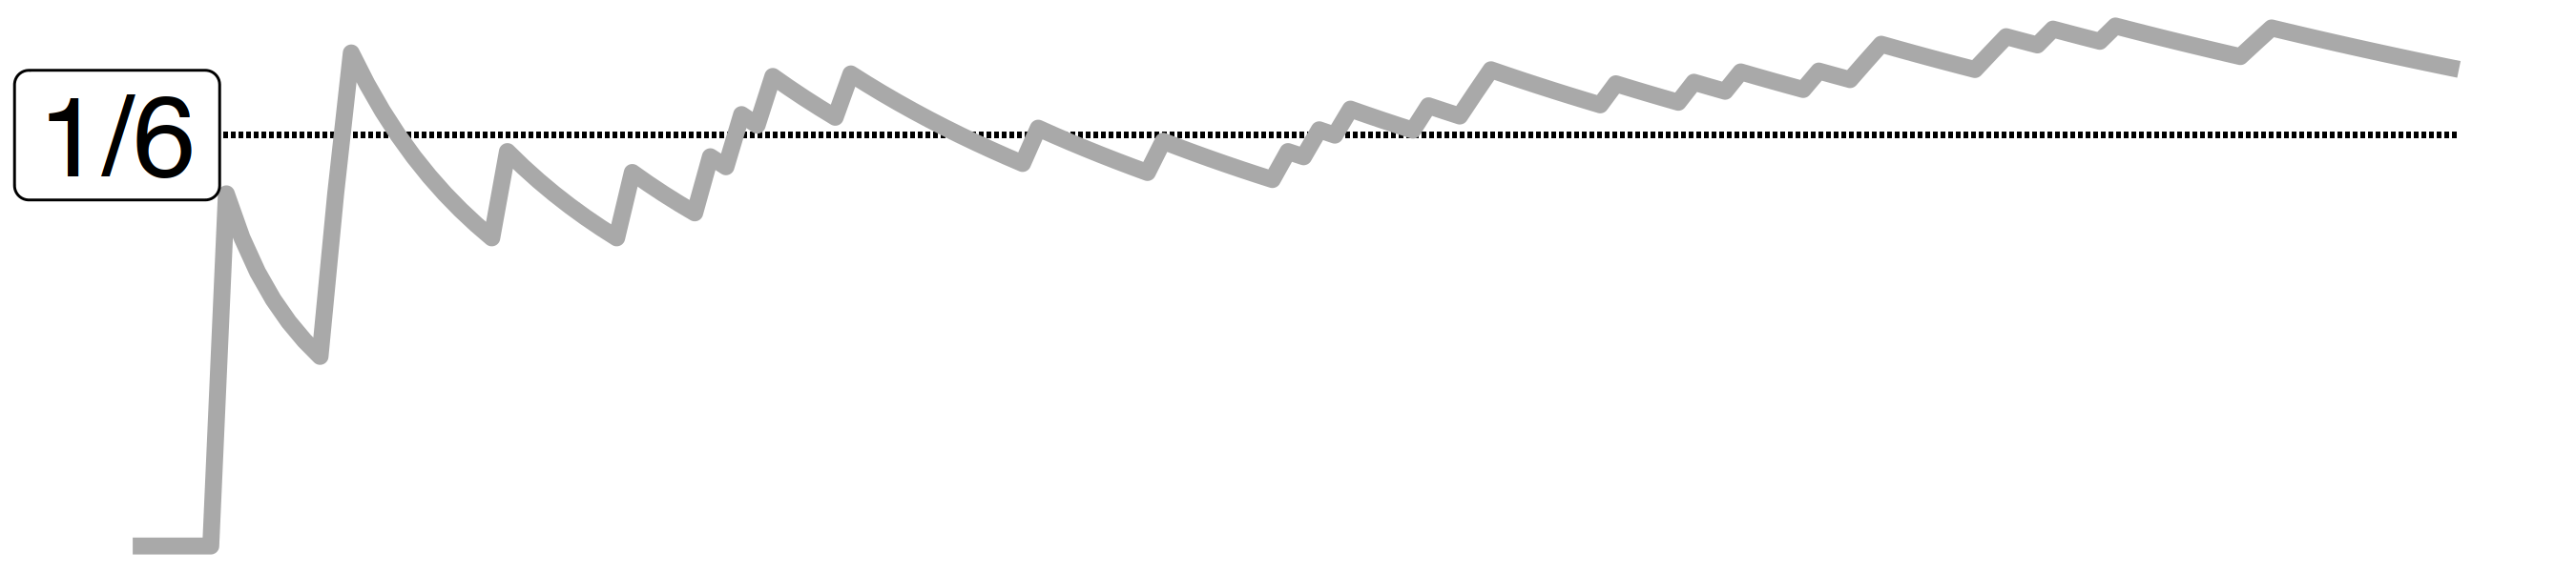
\includegraphics[width=0.8\textwidth]{figures/dice-1} 

}

\caption{The line shows how the relative frequency of 6 eyes changes as the number of dice roles increases from 1 to 100 (left to right).}\label{fig:dice}
\end{figure}

Imagining experiments that will never take place is essential to the frequentist mindset.
By defining probability in terms of long-run frequencies, the entire mindset requires imagining that the sampling and experiment will be done many times.
These ``imagined'' experiments are central to the interpretation of confidence intervals, p-values, and hypothesis tests.

These imagined experiments have a curious implication for frequentism.
Frequentism violates the likelihood principle, which says that all evidence about the data is contained in the likelihood function.
But with frequentism, it's important to know what experiments we are further imagining.
You can find a simple example involving coin tosses in the \protect\hyperlink{likelihoodism}{Likelihoodism chapter}.
In contrast, both \protect\hyperlink{likelihoodism}{Likelihoodism} and \protect\hyperlink{bayesianism}{Bayesianism} adhere to the likelihood principle.

\hypertarget{estimators-are-random-variables}{%
\section{Estimators are Random Variables}\label{estimators-are-random-variables}}

We can learn a lot about frequentist inference, especially in contrast to Bayesian inference, by understanding which ``things'' are random variables and which are not.
In the frequentist mindset, the estimand, the ``true'' but unknown parameter is assumed to be fixed.
Mean, variance and other distribution parameters, model coefficients, nuisance parameters, all are seen as having some unknown but fixed value.
And the values can be uncovered with frequentist inference.
Bayesians, in contrast, view all these parameter as random variables.

Since the quantities of interest are seen as fixed but unkown, the frequentist's job is to estimate them from data.
The estimation is done with a statistical estimator: A mathematical procedure for inferring the estimand from data.
The estimator is a function of the data.
And data are realizations of random variables.
The consequence is that also the estimators themselves are random variables.
Again, we can contrast this with Bayesian mindset:
Bayesians assume that the parameters are random variables.
Bayesians simply update the (prior) probability distribution of the parameters and get new (posterior) probability distributions.

Typical frequentist constructs like confidence intervals, test statistics and p-values are also random variables.
Mix this with the long-run frequencies and you get a special interpretation, for example, for \protect\hyperlink{confidence-intervals}{confidence intervals}.

Let's say you want to know how many teas you drink on average per day.
If you were frequentist, you would assume that there is a true but unknown average number of teas.
Let's call this estimand \(\lambda\).
The frequentist might assume that the daily number of teas follows a Poisson distribution.
The Poisson distribution can handle count data well, and is described by the ``intensity'' \(\lambda\) with which events happen.
Conveniently, the intensity parameter \(\lambda\) is also the expected number of events.
Teas in our case.
We could estimate the tea intensity using the maximum likelihood estimator: \(\hat{\lambda}= \frac{1}{n} \sum_{i=1}^n k_i\), where \(k_i\) is the number of teas on day \(i\).
Our estimator \(\hat{\lambda}\) is a random variable.
If the model assumptions are correct and if the world is truly frequentist, then the estimator \(\hat{\lambda}\) will get closer and closer to the true \(\lambda\) as \(n\) increases.
\(\hat{\lambda}\) approximately follows a Normal distribution.

Frequentist inference builds on the fact that the estimators are random variables.
Combined with the idea of fixed true parameters, it becomes possible to connect the analysis results to the real world.
A commonly used tool to derive insights about the world is null hypothesis significance testing.

\hypertarget{null-hypothesis-significance-testing}{%
\section{Null Hypothesis Significance Testing}\label{null-hypothesis-significance-testing}}

Let's say, your estimator \(\hat{\lambda}\) says that you drink 2.5 teas per month on average.
Initially you had the hypothesis that you drink 3.0 teas per month.
Obviously \(2.5 \neq 3.0\), so the initial hypothesis is incorrect.
Case closed.
But that would be too simple an answer, wouldn't it?
You also wouldn't say that a coin is unfair if heads come up in 51/100 tosses just because \(51 \neq 50\).
But when would a frequentist reject the initial hypothesis of 3.0 teas?
Would we reject the hypothesis if we get \(\hat{\lambda}<2.9\), or \(\hat{\lambda}<2.5\) or maybe must it be much lower, like \(\hat{\lambda}<1.5\)?
Only with the \protect\hyperlink{statistical-modeling}{statistical modeling mindset} we can't answer this question.

The frequentist mindset has an answer to this question of whether to accept or reject a hypothesis.
The frequentist estimator for the number of teas is a random variable that is supposed to approximate the true number of teas.
We can make (frequentist) probabilistic statements about this estimator.
And while the true value for \(\lambda\) is unknown, we can study the hypothesis of \(\lambda = 3.0\) by examining the random variable \(\hat{\lambda}\).

This idea of proposing a hypothesis, and then accepting or rejecting it based on a statistical model or test is called null hypothesis significance testing.
Hypothesis testing is a central method in the frequentist modeling mindset.
Hypothesis tests simplify decisions:
The frequentist accepts or rejects the so-called null hypothesis based on the results of the statistical model.
A statistical model can be very simple:
It can be as simple as assuming that the data follow a Normal distribution and comparing two means with a Student t-test.

How do these hypothesis tests work?

\begin{itemize}
\tightlist
\item
  Start with a hypothesis.
\item
  Formulate the \textbf{alternative/null hypothesis}.
\item
  Decide which statistical test to use. This step includes modeling the data.
\item
  Calculate the distribution of the parameter estimates under the null hypothesis (or rather, the test statistic \(T\)).
\item
  Choose the significance level \(\alpha\). \(\alpha\) is the probability threshold at which to reject the null hypothesis even if it's true. Often \(\alpha = 0.05\).
\item
  Calculate the p-value: p is the probability of observing a more extreme estimate than what is actually observed. See figure \ref{fig:hypothesis}.
\item
  If \(\text{p-value} <\alpha\), then the null hypothesis is rejected.
\end{itemize}

Some examples of tests and test statistics:

\begin{itemize}
\tightlist
\item
  Comparing the means of two distributions. Do Germans consume more pretzels than U.S. Americans? Hypothesis: Germans eat more pretzels. The ``model'' of the data simply assumes a Normal distribution for average pretzels consumption per person. The null hypothesis would be that Germans and U.S. Americans consume the same amount. Then we would run a t-test. The test statistic in the t-test is the (scaled) difference of the two means.
\item
  Estimating the effect of one variable on another. Is surgery better than physiotherapy for treating a torn meniscus in your knee? The statistical model can a linear regression model. The model could predict knee pain dependent on whether a patient had physiotherapy or surgery. The null hypothesis would be that there is no difference in pain, so a model coefficient of zero for surgery/physiotherapy. The test statistic \(T\) would be the coefficient divided by its standard deviation.
\end{itemize}

The p-value has a frequentist interpretation because it is based on long run frequencies.
The p-value is interpreted as the probability that we would observe a more extreme outcome than the one we observed under the null hypothesis.
Again, the frequentist interprets probability with imagined future experiments.
A p-value of 0.03 for an estimated average of 3.0 daily teas would mean the following:
If we repeat the analysis many times and the null hypothesis \(\lambda = 2\) is correct, 3\% of the time we would observe an estimate of \(\hat{\lambda} \geq 3\).
If \(\alpha = 0.05\) was chosen, the null hypothesis would be rejected.

\begin{figure}

{\centering 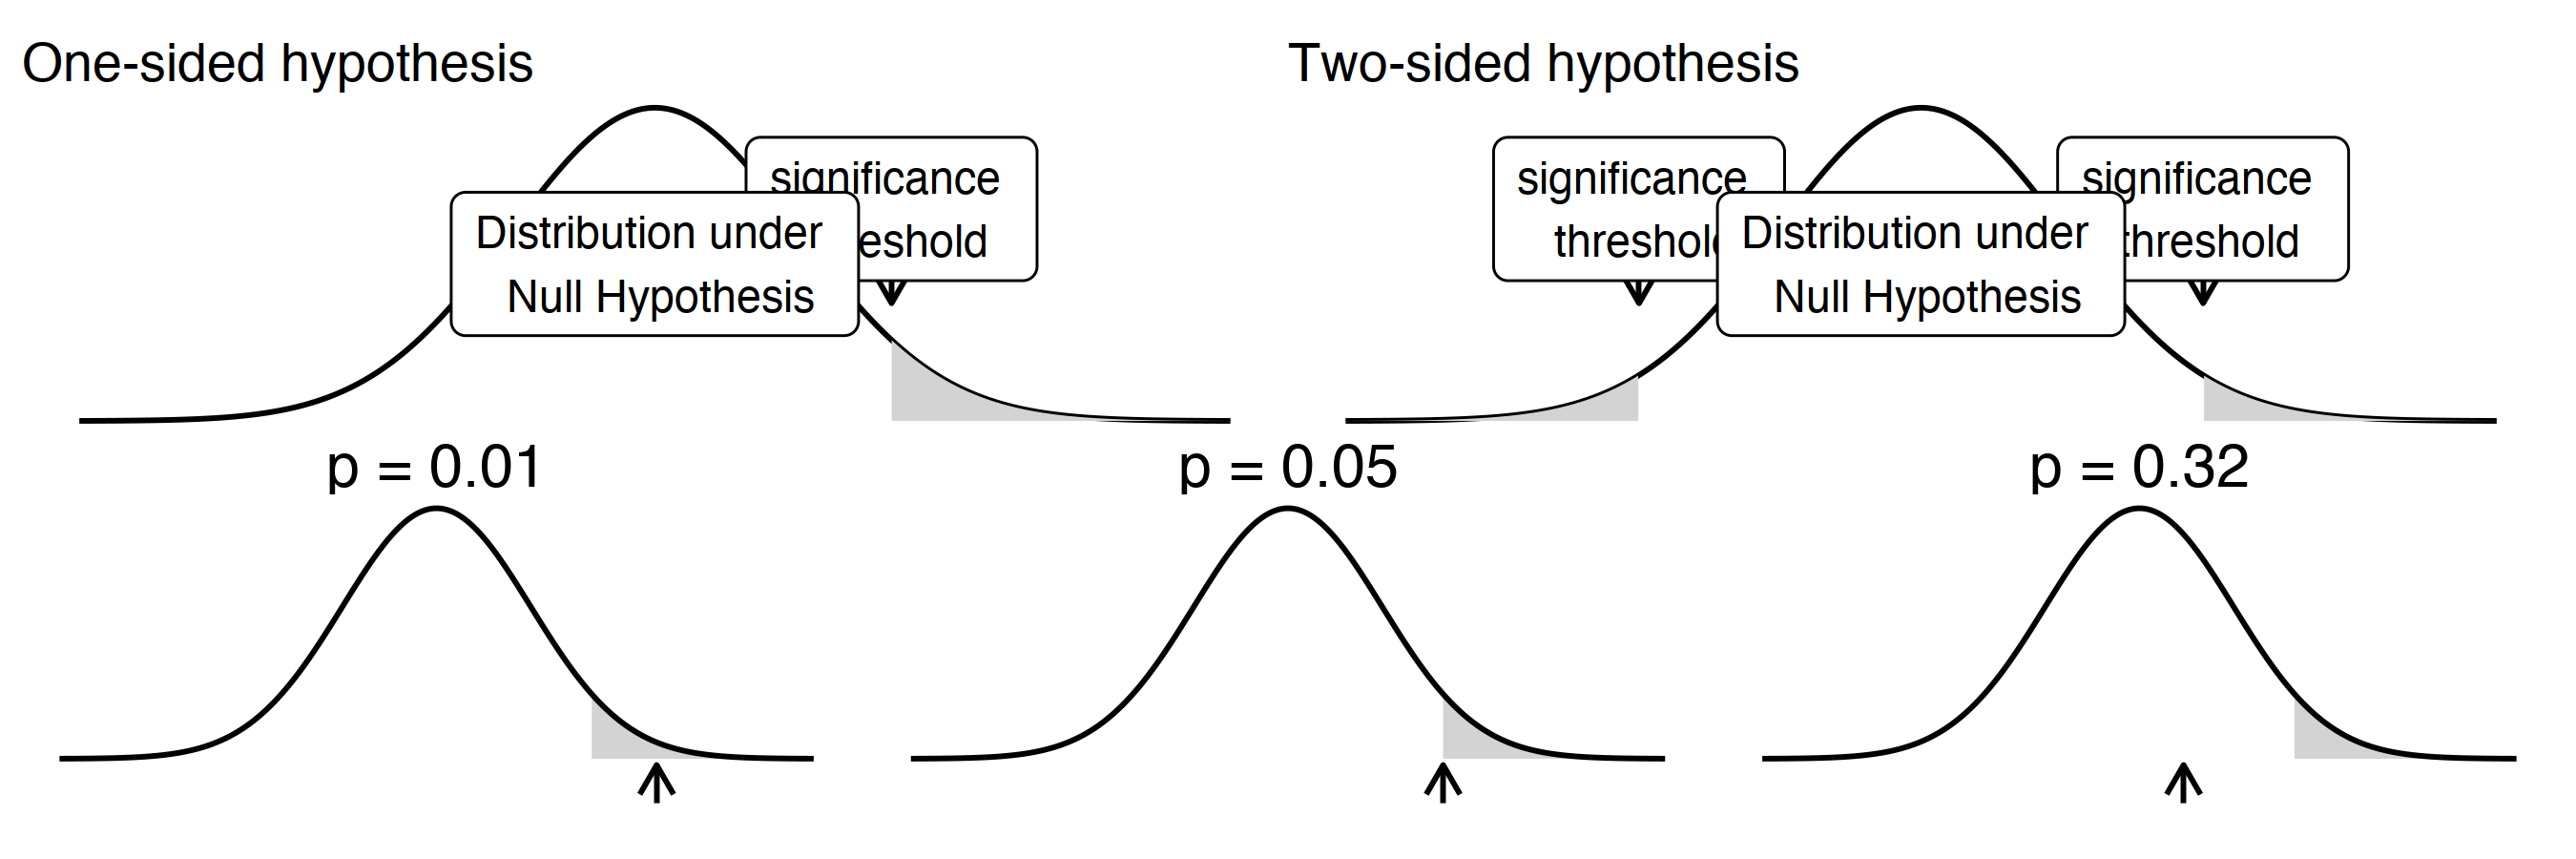
\includegraphics[width=0.8\textwidth]{figures/hypothesis-1} 

}

\caption{Frequentists make binary decisions based on hypothesis tests. Assuming the null distribution, the null hypothesis is rejected if the observed estimand is extreme.}\label{fig:hypothesis}
\end{figure}

Null hypothesis testing is very weird.
It's like answering the question around two corners.
Let's say a researcher wants to prove that a drug prevents migraines.
They test the drug because they expect it to work, so the hypothesis they assume to be true is that patients that take the drug have fewer migraines.
But the null hypothesis is formulated the other way around:
The null hypothesis assumes that the drug has no effect.
Suddenly the goal of the researcher becomes to show that the null hypothesis is false, rather than showing that their hypothesis is correct.
The problem with statistical models is: We can't prove that they are true because our assumptions are not testable.
With frequentist inference, however, we can tell how likely a model result is under a given hypothesis and given the data.
That's why hypothesis tests work by rejection.

P-values allow simple decisions: Is the parameter different from zero?
If yes, frequentists speak of significant effects.
Unfortunately, the entire modeling process is often ultimately reduced to the question of statistical significance.
Achieving a significant result becomes the ultimate goal of a researcher's analysis.
Chasing those small p-values.

\hypertarget{confidence-intervals}{%
\section{Confidence Intervals}\label{confidence-intervals}}

Frequentists use confidence intervals as an alternative to statistical tests.
Hypothesis tests and confidence intervals ultimately lead to the same decisions, but confidence intervals are more informative.
Many statisticians prefer confidence intervals over mere p-values.

Remember that estimators, such as model parameters, are random variables?
That means that estimators have probability distributions.
A confidence interval describes where the mass of that distribution lies.
What percentage of the distribution we want in the confidence interval is again decided by the modeler using an \(\alpha\)-level.
If \(\alpha = 0.05\), then we get a 95\%-confidence interval.
The construction of the confidence interval depends on the probability distribution we have derived for the quantity of interest (coefficient, mean estimate, \ldots).

How are the confidence intervals to be interpreted?
Well, in a frequentist manner, of course!
The ``true'' parameter value is fixed, so it's not a random variable.
To say that the true parameter is in the confidence interval with a 95\% probability would be false.
The true parameter is either in the interval or it's not, we just don't know.
The confidence itself is a random variable since it's derived from data and therefore from other random variables.
So the interpretation of a 95\% confidence interval is:
If we were to repeat the analysis many times, the confidence interval would cover the true value of the quantity of interest 95\% of the time.
Only given that the model assumptions are correct.
As you can see, this is a very frequentist point of view: the confidence interval is interpreted in the context of repeated experiments.

Confidence intervals look different from tests at first glance.
But they are equivalent to the tests:
At least you get the same accept/reject result for the same significance level \(\alpha\).
But the confidence interval contains more information than a simple hypothesis test.
The interval gives the estimate, and lower and upper bounds.
This gives the modeler a better sense of the estimate and its uncertainty.
Rejection of the null hypothesis is equivalent to the null hypothesis being outside of the confidence interval.

\begin{figure}

{\centering 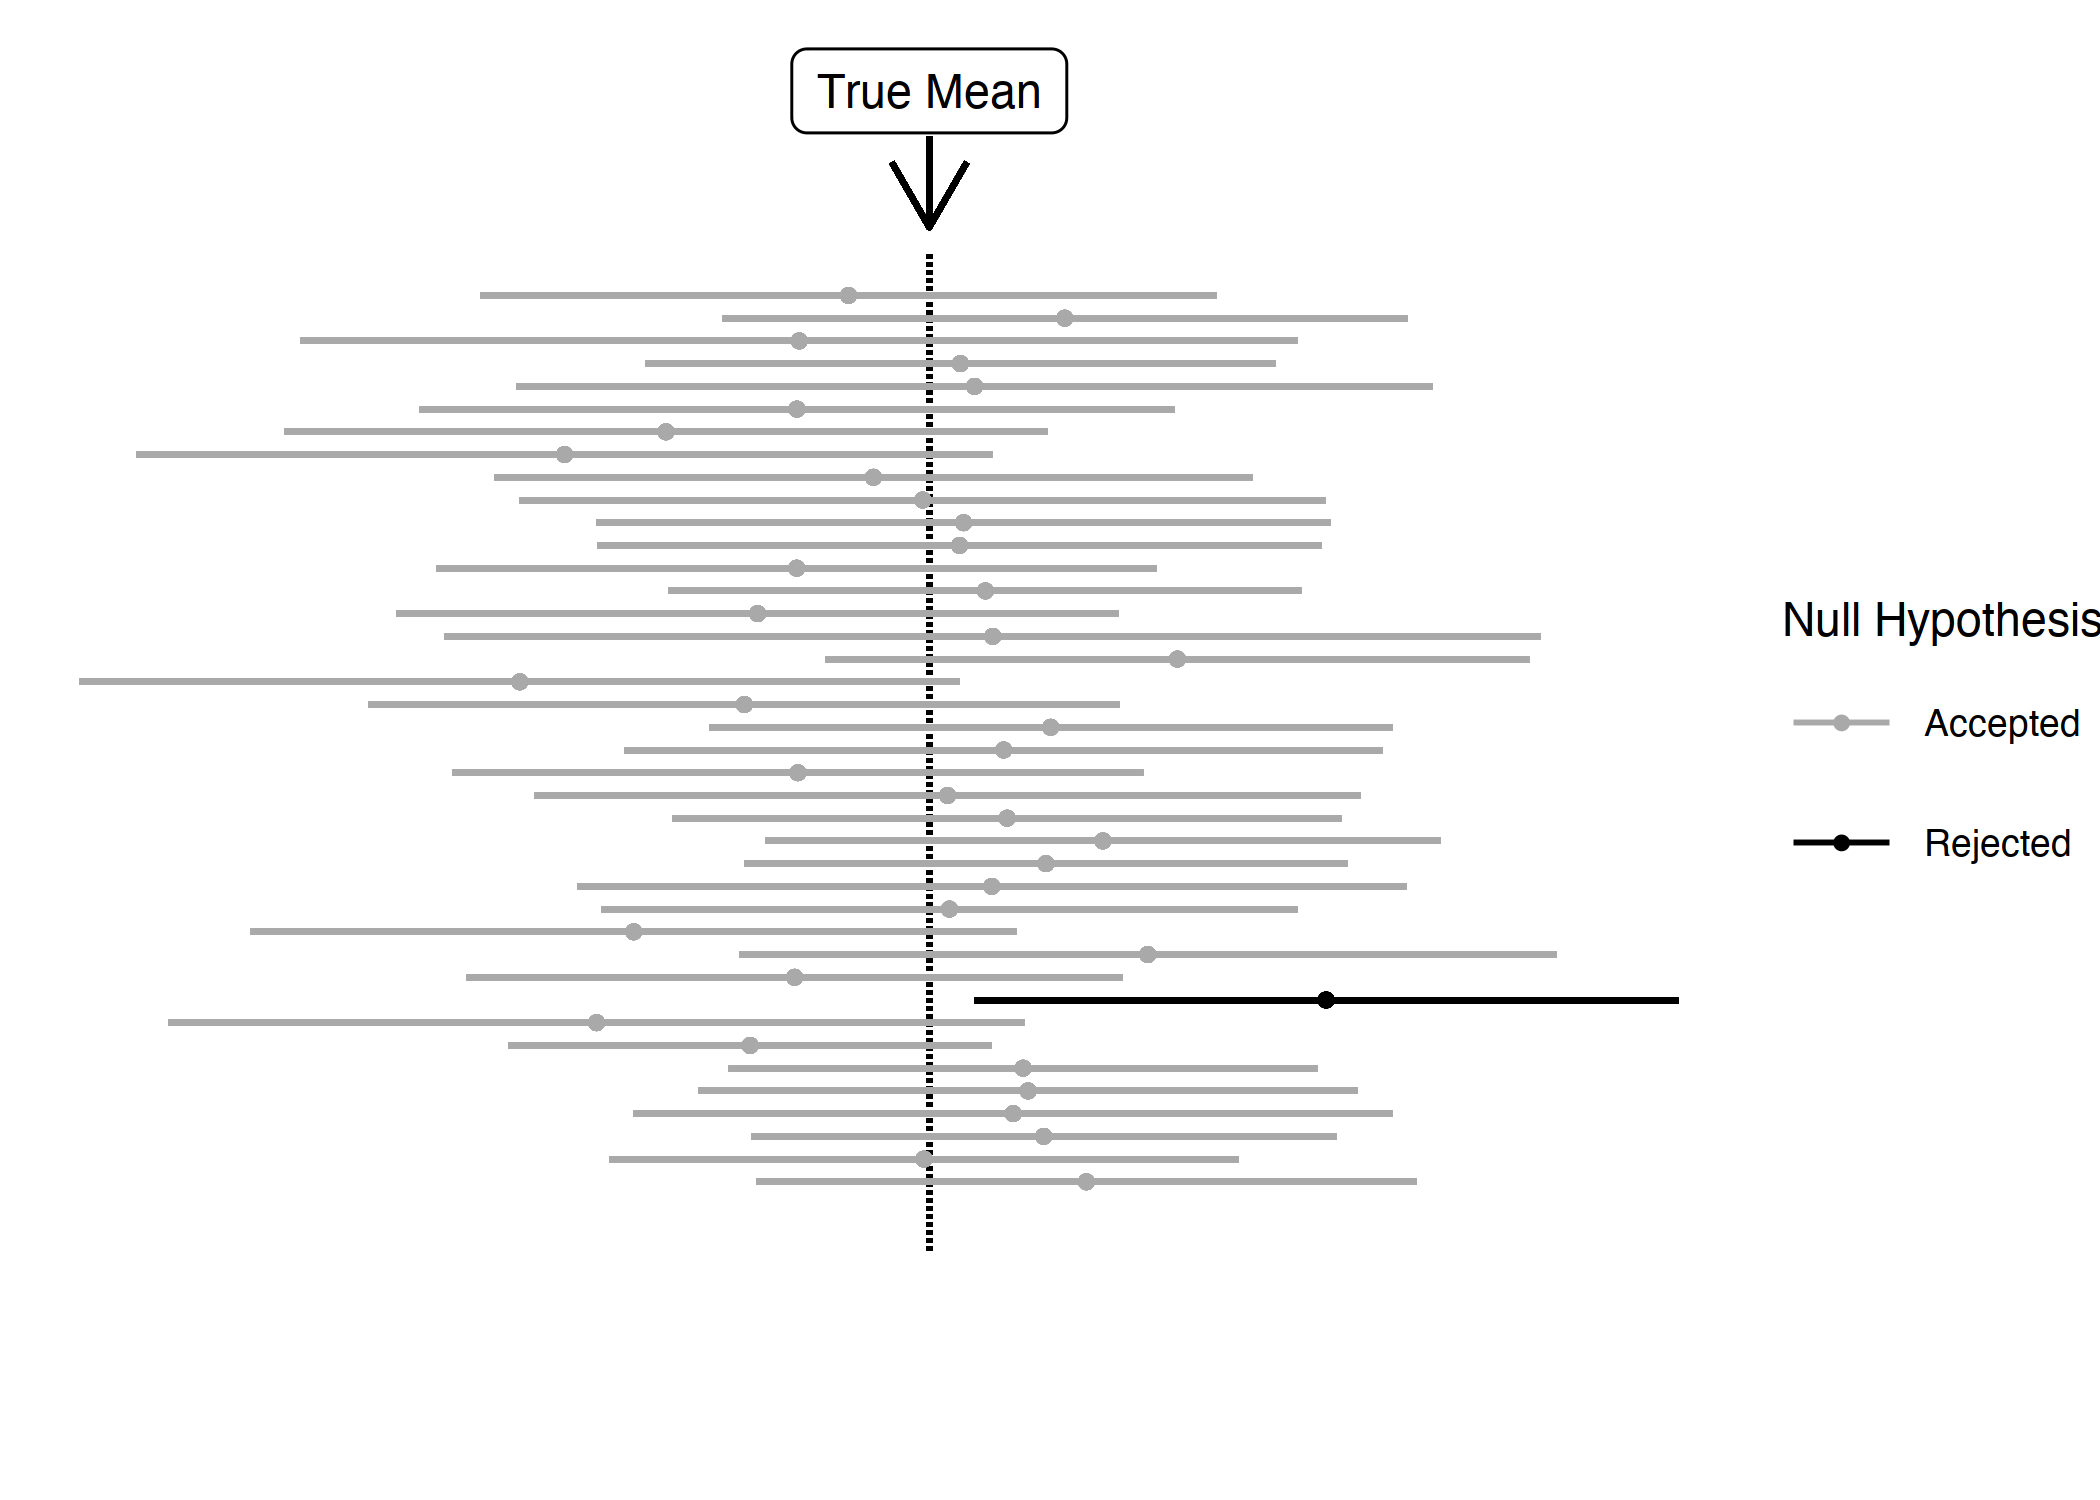
\includegraphics[width=0.8\textwidth]{figures/ci-1} 

}

\caption{100 95\% confidence intervals and the true value.}\label{fig:ci}
\end{figure}

-\textgreater{}

\hypertarget{strengths-1}{%
\section{Strengths}\label{strengths-1}}

\begin{itemize}
\tightlist
\item
  Once you understand frequentist inference, you have the key to understanding most modern research findings. I studied statistics and can now quickly grasp many research papers. For example, to figure out whether I should have knee surgery for my torn meniscus, I read papers comparing knee surgery and physiotherapy alone. All of those papers used frequentist methods, and although I didn't understand everything, I was able to quickly get an idea of their analyses and results.
\item
  Frequentist methods are generally faster to compute than \protect\hyperlink{bayesian}{Bayesian inference} or \protect\hyperlink{supervised-ml}{machine learning}.
\item
  Compared to \protect\hyperlink{bayesian}{Bayesianism}, no prior information about the parameters is required. This makes frequentism more objective.
\item
  Frequentism allows binary decisions (accept/reject hypothesis). This simplicity one of the reasons why it's so popular for scientists and why managers love it.
\item
  Frequentism has all the advantages of the \protect\hyperlink{statistical-modeling}{statistical models} in general: a solid theoretical foundation and an appreciation of the data-generating process.
\item
  When the underlying process is a long-run, repeated experiment, frequentist inference shines. Casino games, model benchmarks, \ldots{}
\end{itemize}

\hypertarget{limitations-1}{%
\section{Limitations}\label{limitations-1}}

\begin{itemize}
\tightlist
\item
  Frequentism invites \textbf{over-simplification of answers}into simple yes/no-answers. Simplification into the question of results ``significantly'' deviate from the null hypothesis. Reducing models to binary decisions obscures critical model assumptions and the difficult trade-offs that had to be made for the analysis.
\item
  Focusing on p-values encourages \textbf{p-hacking}: the either conscious or unconscious search for ``positive'' results. Guided by the lure of a significant result, researchers and data scientists may play around with their analysis until the p-value in question is small enough. With \(\alpha\)-level of 0.05, 1 in 20 null hypotheses are falsely rejected. P-hacking increases this percentage of false positive findings.
\item
  Similarly, if the analysis is exploratory rather than hypothesis-driven, a naive frequentist approach may produce many false positive findings. Look again at figure \ref{fig:ci}: Imagine these were confidence intervals for different variables. Again, for \(\alpha = 0.05\), we would expect 1 in 20 hypothesis tests to yield false positives. Now imagine a data scientist testing hundreds of hypothesis tests. This problem is called the multiple testing problem. There are solutions, but they are not always used and multiple testing can be very subtle.
\item
  The frequentist interpretation of probability is very awkward when it comes to confidence intervals and p-values. They are commonly misinterpreted. Arguably, frequentist confidence intervals are not what practitioners want. \protect\hyperlink{bayesian}{Bayesian} credibility intervals are more aligned with the natural interpretation of uncertainty.
\item
  Frequentist analysis depends not only on the data, but also on the experimental design. This is a violation of the likelihood principle that says that all information about the data must be contained in the likelihood, see example in \protect\hyperlink{likelihoodism}{chapter on likelihoodism}.
\item
  Frequentist probability can fail in the simplest scenarios: Imagine you are modeling the probability of rain in August. The data only has 20 August days, all of which are without rain. The frequentist answer is that there is absolutely no chance that it will ever rain in August. The frequentist recommendation is that to collect more data if we want a better answer. \protect\hyperlink{bayesian}{Bayesianism} offers a solution to involve prior information for such estimates.
\item
  There is an ``off-the-shelf''-mentality among users of frequentist inference. Instead of carefully adapting a probability model to the data, an off-the-shelf statistical test or statistical model is chosen. The choice is based on just a few properties of the data. For example, there are popular flow charts of choosing an appropriate statistical test.
\item
  Frequentist statistics says nothing about causality except that ``correlation does not imply causation''.
\end{itemize}

\hypertarget{bayesian}{%
\chapter{Bayesian Inference}\label{bayesian}}

Bayesian inference sees the world as parameterized distributions.
To learn about the world, we have to learn about the best fitting parameters.
But for Bayesians, the parameters themselves are random variables with a probability distribution.
So to learn about the parameters, we have to assume some prior distribution, and update our belief about the our parameters with data.
This is then the posteriori distribution.

Bayesian inference is a likelihood-based apprach that builds on the Bayes theorem:
The distribution parameters do not only depend on the data, but we assume some prior distribution.
In Bayesian statistics, probability can be interpreted as the plausibility of an event.
Bayesian statistics is about the degree of beliefs we have about our parameters.
Bayesianism is therefore found on the idea of subjective probabilities.
If you haven't read the \protect\hyperlink{statistical-inference}{chapter on statistical inference}, I recommend you do it first, since Bayesian inference is easier understood when you have a good grasp on statistical inference.
The core difference to frequentism are: Heavy use of Bayes' theorem; assumption of prior distribution of parameters; interpretation of probability as degrees of beliefs and not as long-run frequencies.

Bayesian inference is about changing your mind.
We update our knowledge about the world when new information comes in.
You already know some stuff to the world.
Prior to getting some new information.
Then you update your knowledge, based on data / evidence.
Then you go about your life with this udpated knowledge.

Imagine you are at a snack machine.
You have a general idea how much you like snack machines.
You rate most snack vending machines 6/10 - 9/10.
Without further knowledge, you would expect the new machine that you just encountered to be somewhere in that range too.
But this newly installed machine is directly at the train station, and it has your favorite chips.
So you give it a rating of 9/10.
But then two big betrayals.
First, the chips got stuck one day, between the tray and the window pane.
This happens, but it's always very annoying.
But directly the day after, the machine refused to give you change.
These betrayals made you change your rating to 5/10.

\hypertarget{bayes-theorem}{%
\section{Bayes Theorem}\label{bayes-theorem}}

At the very center of Bayesian inference is the Bayes' theorem.
The Bayes' theorem expresses a conditional probability in terms of other probabilities.
As such, the theorem has many applications.

In the case of Bayesian modelling, we are interested in the distribution of the parameters \(\theta\) conditional on the data \(D\), which is \(P(\theta | D)\).
So far, equivalent to \protect\hyperlink{frequentism}{frequentism} and \protect\hyperlink{likelihoodism}{likelihoodism}, with the difference that Bayesians explicitly say that the model parameters \(\theta\) are random variables and therefore have probability distributions.
To
Applying the Bayes' theorem:

\[\underbrace{P(\theta|D)}_{\text{posteriori}} = \frac{\overbrace{P(D | \theta)}^{\text{likelihood}} \cdot  \overbrace{P(\theta)}^{\text{priori}}}{\underbrace{P(D)}_{\text{evidence}}}\]

The Bayes' theorem in the context of Bayesian inference contains the idea of belief updates, as also visualized in Figure \ref{fig:bayesian}.
\(P(\theta)\), also called the prior, is the probability distribution of \(\theta\) before we have collected any data.
The probability distribution gets updated by multiplying the prior with the likelihood \(P(D | \theta)\) of the data.
This product is scaled by the probability of the data \(P(D)\), also called evidence.
The result is the posteriori probability distribution, an updated belief about our parameters \(\theta\).

\begin{figure}

{\centering 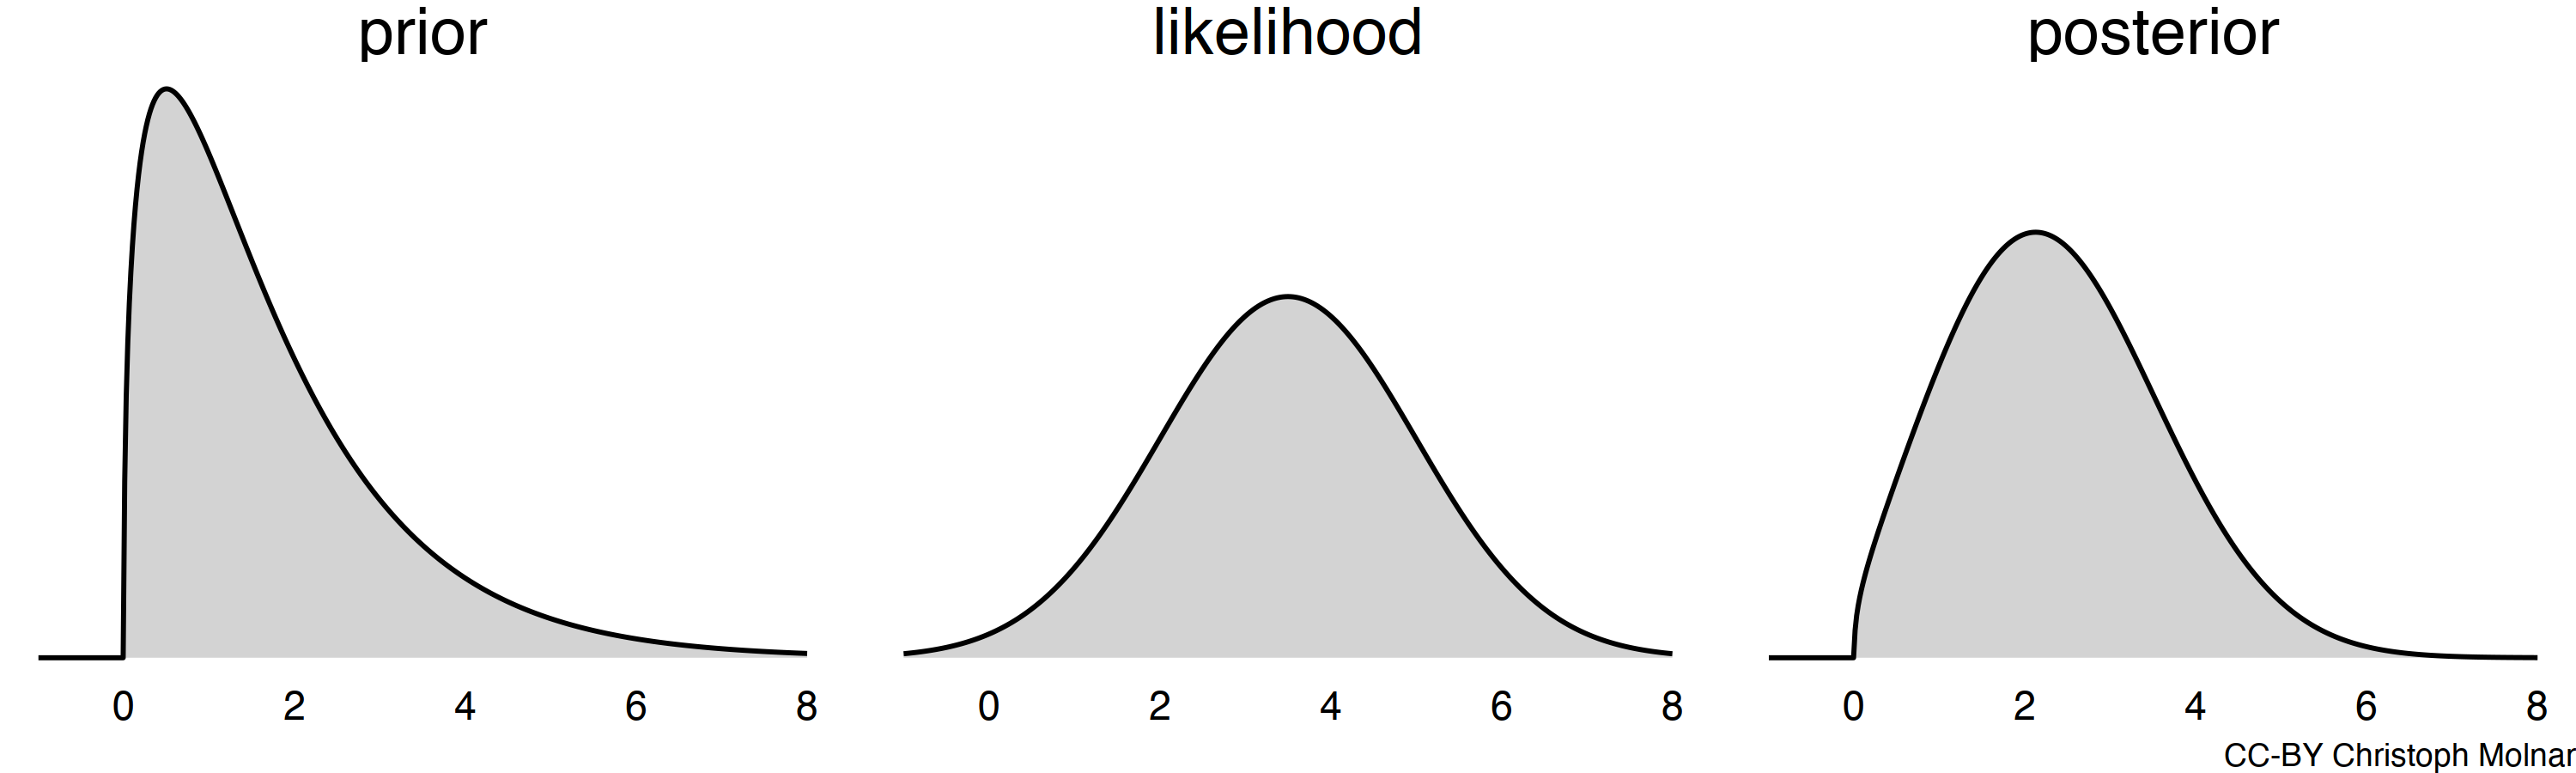
\includegraphics[width=0.8\textwidth]{figures/bayesian-1} 

}

\caption{Illustration of priori density that gets an update from the likelihood of the data to result in posteriori probability distribution.}\label{fig:bayesian}
\end{figure}

Next, let's dive deeper into the individual components of the Bayes' theorem, so that we can update our own beliefs about Bayesianism.

\hypertarget{prior-probability}{%
\section{Prior Probability}\label{prior-probability}}

The Bayes' theorem tells us that we have to know \(P(\theta)\) to calculate the posterior probability distribution.
This implies that the model parameters themselves are random variables, or otherwise \(P(\theta)\) is a meaningless statement.
For example, the mean of a distribution has a distribution itself.
Let's sat we randomly choose a person and want to know how long they worked today.
The number of daily working hours, the random variable of interest, follow some probability distribution that have parameters.
For example, it might follow a Gaussian distribution, which is described with mean and variance parameters.
Bayesians would assume that the mean parameter is itself a random variable.

How would we know how the model parameter is distributed, when we haven't even observed any data yet?
Bayesians assume some prior distribution.
The factors going into the choice of prior distribution are manifold.
The clearest factor are constraints on the space the parameter lives in:
Is the parameter the mean of distribution? Then we need a continuous distribution, for example Gaussian.
Maybe you know that the mean is positive, so you pick a prior distribution that only contains positive values, for example the Gamma distribution.
Furthermore, expert knowledge can be used to inform the choice.
Maybe we know from other experiments that the mean of the data distribution should be near 1.
So we could assume a Normal distribution for \(\theta\): \(\theta \sim N(1, 1)\).
In the case of Binomial distribution of your data, for binary outcomes, the Beta distribution is a good prior (see Figure \ref{fig:priors}).
Depending on your belief about the parameter \(\pi\) you might choose a very different parameteriziation of the Beta distribution.
Maybe you belief the parameter to be symmetrically distributed around 0.5.
Or maybe the parameter is more drawn to 0.25?
Another Beta prior might put emphasis on \(\pi\) being one.
But it's also possible to have a prior that puts most probability on 0 and 1 symmetrically.
When there are no specific prior beliefs about the parameter the Bayesian can use an ``uninformative'' or ``objective'' priors, meaning \footnote{Yang, Ruoyong, and James O. Berger. A catalog of noninformative priors. Durham, NC, USA: Institute of Statistics and Decision Sciences, Duke University, 1996.}
Another factor is mathematical convenience.
It's convenient to pick conjugate priors.
A convenient case is using conjugate priors.
Conjugate priors are probability distributions that remain of the same family when combined with certain likelihood functions.
Suppose you model your data as Bernoulli distribution, which describes the distribution as probabilities of being 1 with probability of \(p\) and 0 otherwise.Then we measure a realization \(X\) of this Bernoulli random variable.
Further, if we assume to have a Beta distribution as prior distribution, then we also have a beta posteriori function.

The reliance on choosing prior probability functions is the Achilles' heel of Bayesianism, or at least the biggest target of critique.
The subjective choice of a prior probability influences all results coming from Bayesian inference.
It clashes especially with the frequentist mindset that there is some true and constant parameters out there.
And frequentist aim to be very objective, by only operating on long-run frequencies.
Also likelihoodism says that all information is in the likelihood, which clashes with the idea of a prior distribution influencing the outcome.

However, there are two major objections to this criticism.
First, the more data we have, the less influential the prior distribution becomes.
And second, the prior is not hidden or anything, influencing the analysis from the shadows.
Let's say two experts disagree on which prior to use.
You can run Bayesian inference twice, and compare the results.

To get to the posterior likelihood of our parameters, our ultimate goal in Bayesian inferene, we have to update our prior belief with data, or rather: the likelihood function.

\begin{figure}

{\centering 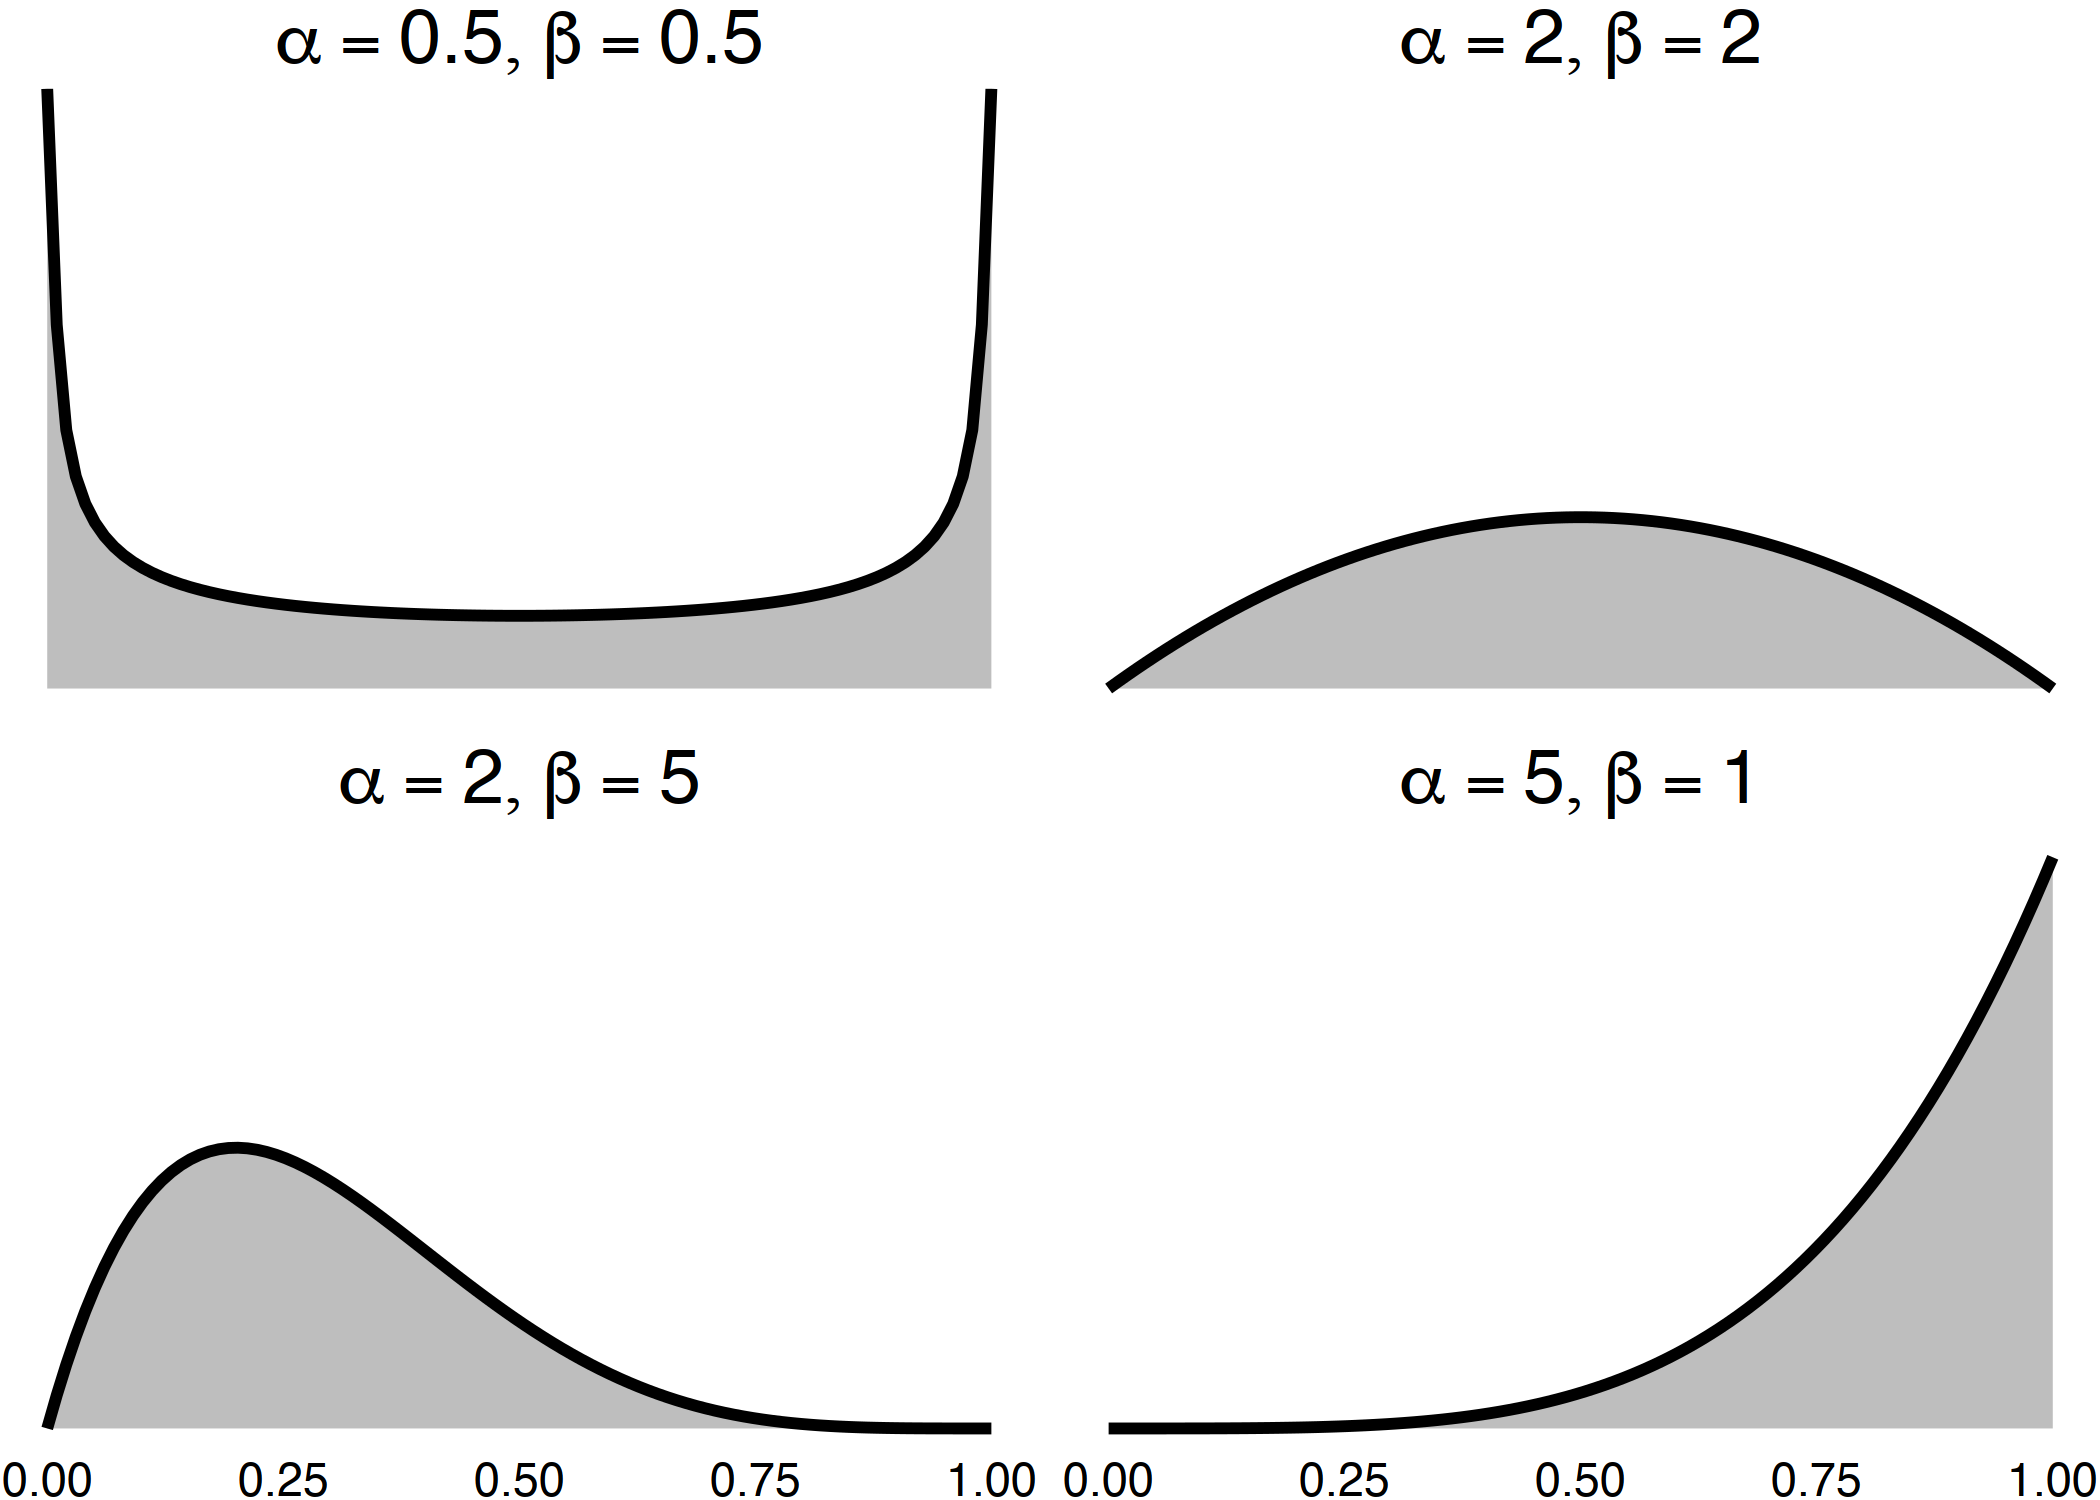
\includegraphics[width=0.8\textwidth]{figures/priors-1} 

}

\caption{Various prior distributions for the success probability p in a Binomial ditribution. Priors here are Beta distributions with shape parameters $\alpha$ and $\beta$.}\label{fig:priors}
\end{figure}

\hypertarget{likelihood}{%
\section{Likelihood}\label{likelihood}}

If you have read the \protect\hyperlink{statistical-modeling}{chapter about statistical modeling}, you should be familiar with the likelihood function \(P(\theta | D)\).
The likelihood is the probability function of the data, but with a twist:
We switch the role of data and parameters.
The probability function is a function of the data: We put in a data point and the probability function tells us how probable this data point is. Parameters are assumed to be fixed.
The likelihood function is a function of the parameters: We put in the model parameters, and it tells us how likely the observed data is. Data are assumed to be fixed.

To get to the likelihood, we have to make assumptions about how our data is distributed.
Like any \protect\hyperlink{statistical-modeling}{statistical model}!
So we assume parameterized distributions for our data and turn it into a maximization problem: Finding the right parameter that maximize the likelihood.
That's true at least for \protect\hyperlink{frequentism}{frequentism} and \protect\hyperlink{likelihoodism}{likelihoodism}.
But for Bayesians, it's just part of the equation.
But if you are already familiar with likelihoods and so on, then this part of the Bayesian mindset should be very familiar to you.
Another part of the equation is the evidence \(P(D)\), but as we will see, it does not matter that much:

\hypertarget{evidence}{%
\section{Evidence}\label{evidence}}

The evidence is the marginalized probability of our data.
It's sometimes called model evidence.
Marginalized means that we integrate over all possible parameter values.
It's a bit difficult to interpret, but that's not a problem at all.
Due to the marginalization, \(P(D)\) does not depend on the parameters \(\theta\) at all.
Which means that in terms of maximizing the posterior probability, it's just a constant factor.
As we will see later on, we can work around \(P(D)\).
We don't have to compute it to get to the posterior probability.
But it means that we have to employ sampling techniques instead of computing the posterior directly.
That's why the posterior probability is often written as being proportional to the numerator:

\[\underbrace{P(\theta|D)}_{\text{posteriori}} \propto \overbrace{P(D | \theta)}^{\text{likelihood}} \cdot  \underbrace{P(\theta)}_{\text{priori}}\]

So, how do we finally estimate the posterior probability?

\hypertarget{posterior-probability-estimation}{%
\section{Posterior Probability Estimation}\label{posterior-probability-estimation}}

The goal of the Bayesian is to estimate the posterior distributions of the parameters.
Once they have that, they can interpret those distributions, make predictions with the model, draw conclusions.

But how do we estimate the posterior?
Ideally you'd want to have a closed form expression to calculate the posterior.
That's possible in simple cases, for example when you used conjugate priors.
But in many modelling cases, it's not possible to get a closed form expression to calculate the posterior probability distribution.
The problem here is the \(P(D)\).
The evidence is too difficult to compute.
Not only is \(P(D)\) a problem:
Also there can be many parameters, and we have a high-dimensional optimization problem.
So we need to be clever about optimizing it.

We don't HAVE to compute it.
Another option is to just sample from it.
Special sampling techniques from the posterior distribution is the go-to solution to fit the posterior distribution.
A method called Markov Chain Monte Carlo (MCMC) is typically employed for this sampling task

We start with some initial values for our parameters.
Then new parameter values are proposed.
This requires some prooposal function.
These new values are either accepted or rejected, based on prior and likelihood.
If jump is accepted, adapt parameters.
In any case, go back to step 2 of new parameter proposals.
The process is repeated many times, and produces a ``chain'' of samples for each of the parameters.

How does MCMC make any sense?
During the ``jumping'' between parameters, we are actually comparing models.
This if the acceptance function.
The comparison happens by dividing the posteriors of the model with ``old'' parameter values and the one with the newly proposed parameter values.
The evidence \(P(D)\) cancels out.

We cannot use the entire chain as samples from the posteriori distribution.
First, the first view samples are likely far away from the true posteriori and should therfore be ``burned'', meaning you ignore them.
So, maybe the first 1000 of samples are thrown away.
Then, you want independent samples.
But the samples in the chain are dependent on the ones that come before them.
So we have to sample from the chain, and make sure that there are enough values between the samples.
There are diagnosis tools to do this, but we won't go into the details here.
Then you have samples from your posterior distribution.
Those you can visualize with histogram or density plots.

There are many other more sophisticated sampling methods, but for this introduction it is good enough to show MCMC.
Gibbs sampler, Metropolis-Hastings, \ldots{}
All have in common that they are computationally expensive.
So a big part of the daily job as a Bayesian is to wait for those MCMC chains to converge.
At least compared to a frequentist.

A shorter alternative is variational inference \footnote{Blei, David M., Alp Kucukelbir, and Jon D. McAuliffe. ``Variational inference: A review for statisticians.'' Journal of the American statistical Association 112, no. 518 (2017): 859-877.}.
But while MCMC deliver approximately exact estimates of the posterior probability, variational inference is more of a heuristic.

TODO: Visualize the process that is implied by saying that parameters are random variables

\hypertarget{bayesian-inference}{%
\section{Bayesian Inference}\label{bayesian-inference}}

As said before, getting the posterior distribution is the core of Bayesian mindset.
What can we then do with the posterior probability?
What insights can be drawn from the posterior, and how do we link it with the world?

Remember that Bayesians build \protect\hyperlink{statistical-modeling}{statistical models}:
So they try to approximate the data-generating process with a construct of probability distributions of random variables.
These distributions are parameterized, and Bayesians say that these parameters are random variable themselves.
Also, Bayesians think of probability as degrees of belief.
The posterior represents an updated belief about the parameters that represent the real world.

A parameter might reveal to us the distribution of the treatment effect of a cancer drug.
Or a parameter represents the probability distribution of the mean size of a person.
Visualizing the posterior distributions fully reveals the information that we have.
But there are plenty of options as well to summarize the posterior distributions:

TODO: finish up figure with credible interval, mean

\begin{figure}

{\centering 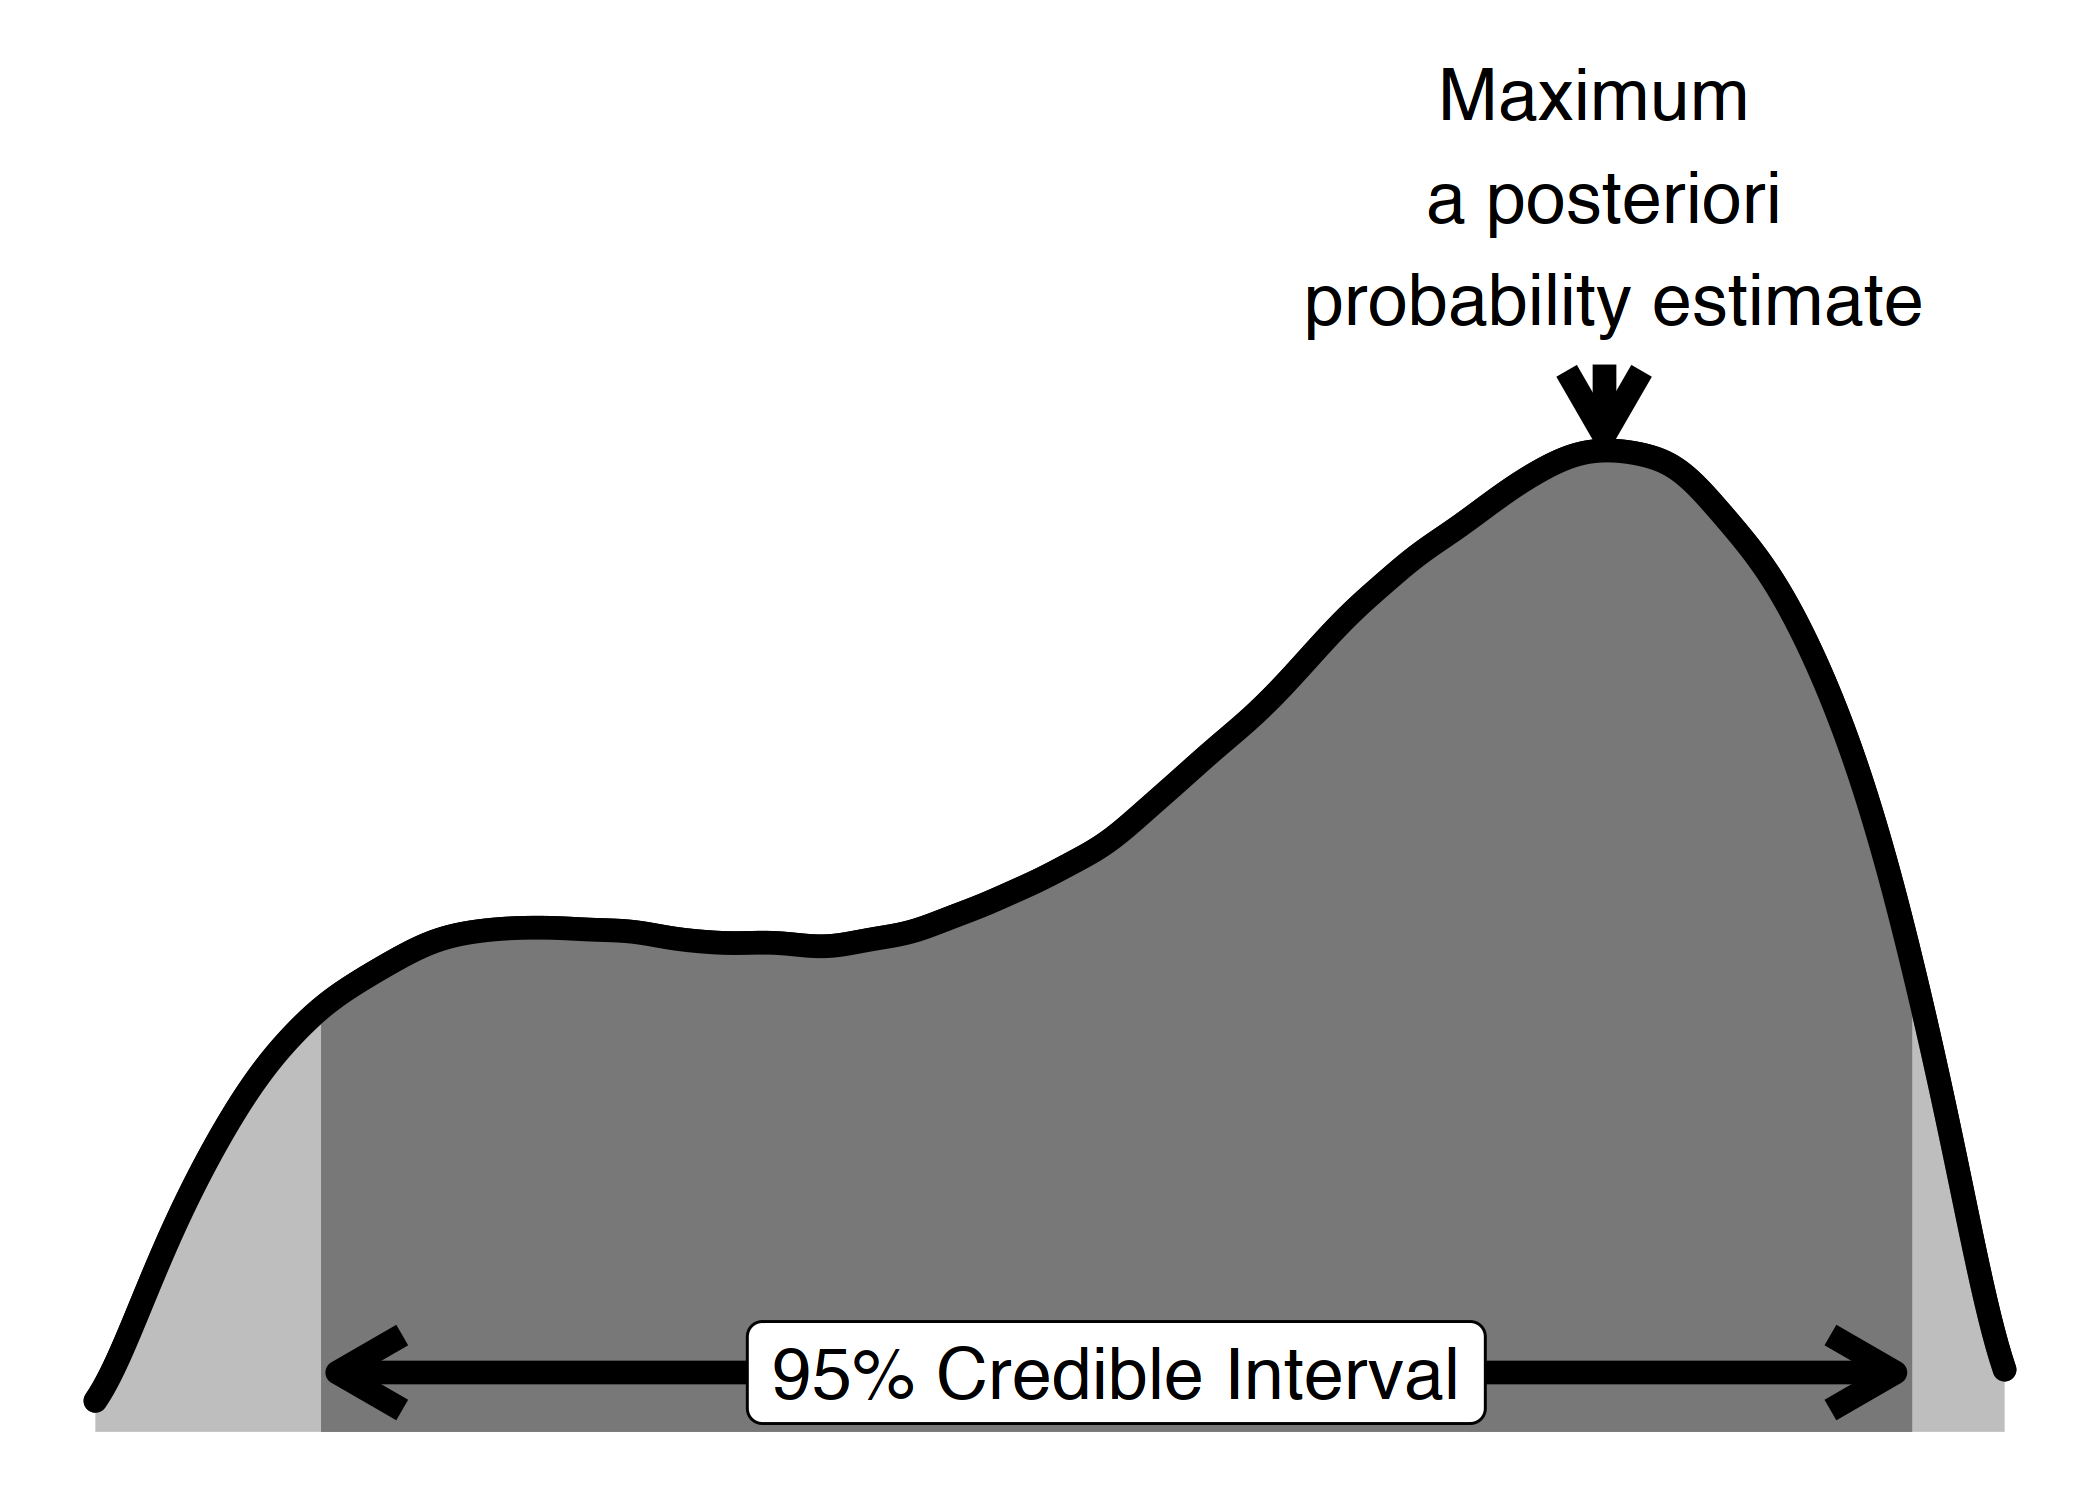
\includegraphics[width=0.8\textwidth]{figures/posteriori-1} 

}

\caption{Describing the posterior distribution.}\label{fig:posteriori}
\end{figure}

Maximum a posteriori estimation: This is the mode (the highest point) of the posteriori distribution. It represents the most likely value.
But there are other summaries:
You could just compute the mean or the median of the posterior probability distribution.
Or any other quantile of the distribution.
Another option are credible intervals.

In frequentist statistics, we get confidence intervals for our estimators.
That's some uncertainty quantifycation telling us how sure we are about our estimation.
But it's different with Bayesian inference.
Since we get posterior probabilities for our parameters, and from the we can derive credibility or credible intervals.
For example, a 95\% credibility interval contains 95\% of the mass of our parameter.
With 95\% probability, the parameter falls within that interval.
Not in the sense that there is some fixed value for the parameter.
But it's a random variable that can take on different values.
Technically, they work the same as confidence intervals in frequentist statistics.
But they have a different philosophical interpretation.

\begin{itemize}
\tightlist
\item
  Since the parameters have a distribution, also the prediction is not just a point-wise prediction.
\item
  posterior predictive distribution: The distribution for a newly predicted data point. To get there, we have to marginalize over the posterior
\item
  IN frequentist statistis, the uncertainty of the model parameters is not regarded in the prediction f a new data point. So it underestimates the variability of the prediction.
\item
  There is also a prior predictive distribution: It's the distribution for a newly predicted data point. But instead of marginalized
\item
\end{itemize}

\hypertarget{strengths-2}{%
\section{Strengths}\label{strengths-2}}

\begin{itemize}
\tightlist
\item
  Bayesianism allows to make use of prior knowledge.
\item
  Priors are especially useful when expert knowledge has to be included in the approach.
\item
  Bayesian inference inherits all advantages of \protect\hyperlink{statistical-modeling}{statistical models}.
\item
  Bayesianism offers an expressive language to build up models
\item
  A natural propagation of variance if, for example, there are uncertainties in the measurement
\item
  A natural appraoch for hierarchical or multilevel modeling.
\item
  Allows a holistic probabilistic approach: Through Bayes' theorem, parameters and data can be chained into a probabilistic model. General solver programs can then automatically derive the posterior estimates using MCMC. Everything is random variable: data and parameters. Everything is tied together by probabilistic operations.
\item
  Thinking like a Bayesian makes you aware of DGP, uncertainties in your parameters, full probability models. Even more than in the frequentist mindset.
\item
  As a more general benefit: Bayesianism is a great mental mdoel for how we update our own hypotheses about the world.
\item
  Arguable a more intuitive interpretation of probability: When practitioners make a wrong interpretation of frequentist confidence interval, what they actually do is interpret them as credible intervals. The interpretation of Bayesian probbility is easier: I believe / it's likely that the parameter is in this area.
\item
  Decoupling of inference and decision. You can first learn those posteriors, and then apply logic to make decision with this inference. Like MAP and credible intervals.
\end{itemize}

\hypertarget{limitations-2}{%
\section{Limitations}\label{limitations-2}}

The most common reasons not to use Bayesian statistics:

\begin{itemize}
\tightlist
\item
  The prior distributions are subjective.
\item
  Bayesian methods are mathematically demanding and computationally expensive (Always waiting for MCMC chains to finish up).
\item
  Not as decisive as frequentism, but can be turned into such with MAP and so on.
\item
  Hard to implement.
\item
  No causal interpretations, just associations.
\end{itemize}

\hypertarget{likelihoodism}{%
\chapter{Likelihoodism}\label{likelihoodism}}

\begin{itemize}
\tightlist
\item
  Focused on the likelihood, follows the likelihood principle.
\item
  Does not assume that parameters are random variables.\\
\item
  A \protect\hyperlink{statistical-modeling}{statistical modeling mindset} with \protect\hyperlink{frequentism}{frequentism} and \protect\hyperlink{bayesianism}{Bayesianism} as alternatives.
\end{itemize}

\textbf{This chapter is under construction! Stay tuned.}

\hypertarget{causal}{%
\chapter{Causal inference}\label{causal}}

\begin{itemize}
\tightlist
\item
  Assumes that random variables are connected through cause and effect.
\item
  Builds a causal model from which statistical estimators are derived.
\item
  A \protect\hyperlink{statistical-modeling}{statistical modeling mindset} that adds causality to \protect\hyperlink{frequentism}{frequentist} and \protect\hyperlink{bayesian}{Bayesian} inference.
\end{itemize}

\textbf{This chapter is under construction! Stay tuned.}

\hypertarget{supervised-ml}{%
\chapter{Supervised Machine Learning}\label{supervised-ml}}

\begin{itemize}
\tightlist
\item
  Focus on prediction rather than understanding the data-generating process.
\item
  Focus on loss minimization and evaluation with unseen data.
\item
  Alternative to the random variable focused \protect\hyperlink{statistical-modeling}{statistical modeling mindset}, but also draws heavily from it, method-wise.
\end{itemize}

\textbf{This chapter is under construction! Stay tuned.}

\hypertarget{deep-learning}{%
\chapter{Deep Learning}\label{deep-learning}}

\begin{itemize}
\tightlist
\item
  Neural networks based on stacking various layers of neurons.
\item
  World of feature embeddings, transfer learning and foundation models.
\item
  A machine learning mindset, can also be used for \protect\hyperlink{supervised-ml}{supervised learning}.
\end{itemize}

\textbf{This chapter is under construction! Stay tuned.}

\hypertarget{design-based-inference}{%
\section{Design-based Inference}\label{design-based-inference}}

TODO

\begin{itemize}
\tightlist
\item
\item
\item
\end{itemize}

\textbf{This chapter is under construction! Stay tuned.}

\hypertarget{references}{%
\chapter*{References}\label{references}}


Blei, David M., Alp Kucukelbir, and Jon D. McAuliffe. ``Variational inference: A review for statisticians.'' Journal of the American statistical Association 112, no. 518 (2017): 859-877.

Gandenberger, Greg. Why I am not a likelihoodist. Ann Arbor, MI: Michigan Publishing, University of Michigan Library, 2016.

Hernán, Miguel A., and James M. Robins. ``Causal inference.'' (2010): 2.

ISyE8843A, Brani Vidakovic Handout. ``1 The Likelihood Principle.''

Ioannidis, John PA. ``Why most published research findings are false.'' PLoS medicine 2, no. 8 (2005): e124.

Judea, Pearl. ``An introduction to causal inference.'' The International Journal of Biostatistics 6, no. 2 (2010): 1-62..

Kao, WH Linda, Ian B. Puddey, Lori L. Boland, Robert L. Watson, and Frederick L. Brancati. ``Alcohol consumption and the risk of type 2 diabetes mellitus: atherosclerosis risk in communities study.'' American journal of epidemiology 154, no. 8 (2001): 748-757.

Pearl, Judea. ``The do-calculus revisited.'' arXiv preprint arXiv:1210.4852 (2012).

Savage, Leonard J. The foundations of statistics. Courier Corporation, 1972.

Some approaches don't assume a closed form distribution. For example the Cox proportional hazards model. For the Cox model, we optimize the partial likelihood. These approaches are called semiparametric.

Weisberg, Michael. Simulation and similarity: Using models to understand the world. Oxford University Press, 2012.

Wynants, Laure, Ben Van Calster, Gary S. Collins, Richard D. Riley, Georg Heinze, Ewoud Schuit, Marc MJ Bonten et al.~``Prediction models for diagnosis and prognosis of covid-19: systematic review and critical appraisal.'' bmj 369 (2020).

Yang, Ruoyong, and James O. Berger. A catalog of noninformative priors. Durham, NC, USA: Institute of Statistics and Decision Sciences, Duke University, 1996.

\printindex
\thispagestyle{empty}


\end{document}
